%%=====================================================
% ロボティックライフサポート研究室
% セミナー資料
%%=====================================================
\documentclass[twocolumn]{jsarticle}

\def\rlsTex{../../rlsTex}
\input{\rlsTex/setup/seminar}

\graphicspath{{../../fig/}{./fig/}}

\seminum{1}
\memonum{R01-01}
\date{2019年05月30日}

\renewcommand{\mpjtitle}{
  DCM/VRP歩行実験に向けた実機モデルによるトルクの検証
}

\renewcommand{\mpetitle}{
 Verification of  the Torques in a DCM/VRP Walking Experiment \\With  HOAP–2 
}

\renewcommand{\mpabstract}{
Various studies have been conducted on gait control of humanoid robots. In this laboratory, gait control in a simulation environment using  the Divergent Component of Motion (DCM) and Virtual Repellent Point (VRP) as an index is realized.
Experiments on a real machine are required for confirmation in a real environment, but careful preparation is necessary to avoid accidents and failures.
In this paper, we examine the joint torque magnitude in Continuous Heel-to-Toe (CHT) gait control, and select the parameters suitable for the experiment.
}

\renewcommand{\mpauthor}{
  平井~春輝
}
\renewcommand{\mpeauthor}{
  Haruki~Hirai
}

\begin{document}
\mtitle



%%%%%%%%%%%%%%%%%%%%%%%%%%%%%%%%%%%%%%%%%%%%%%%%%%%%%%%%%%%%%%%%%%%%%%%% 
% 
% 以下より本文記述
% jpg使用可 $ extractbb test.jpg
% dvi->pdf dvipdfmx test.dvi
% ##############################################
\section{諸言}
人型ロボットの歩行制御において様々な研究がなされいる.また,本研究室でもDCMおよびVRPを指標としたシミュレーション環境での歩行制御が実現されている.
実環境での確認のため実機での実験が求められるが,転倒によるギアの故障や許容トルクを超えることによるモータの破損を回避しなければならない.
よって,許容トルクの確認など慎重な準備が必要である.
本研究では,実環境での適応において人型ロボットの基本動作である二足歩行を,実験機において実現させることを目的とする.
本稿でははじめに,基礎段階として% シミュレーション環境における
二足歩行制御の理論を理解しCHTによる歩行制御の軌道生成を行う.
次に,先行研究での歩行時のトルクの大きさについて検証を行い,実機での歩行を目指すために各パラメータとトルクの大きさとの関係を明確にする.
\section{歩行軌道生成}
\subsection{Cotinuous Double Surpport (CDS)Trajectories}
CDSを用いて,1ステップ先の目標のDCMを与えることで,現在のステップにおける目標VRPから現在のステップ開始時の目標DCMが決定する.
\begin{align}
  \bm{r}_X^{des,i}=
  \bm{r}_{vrp}^{des,i}
  +e^{-\frac{T_{step}}{T_X}}(\bm{r}_{X}^{des,i+1}-\bm{r}_{vrp}^{des,i})
\end{align}
ここで,$T_{step}$はステップ周期である.境界条件が定まり,各ステップ開始時の目標DCMから時刻$t$における目標のDCMの位置が算出可能である.また,時刻$t$におけるDCMの目標速度および加速度はDCMの位置の時間微分により求まる.
さらに,ステップ数が決定しており,最終の目標DCMを与えられる場合,オフラインでの計算が可能である.
\begin{align}
  \bm{r}_X^{des}(t)&= \bm{r}_{vrp}^{des,i}+e^{\frac{(t-T_{step})}{T_X}}(\bm{r}_{X}^{des,i+1}-\bm{r}_{vrp}^{des,i})
  % \\
  % \dot{\bm{r}}_X^{des}(t)&= \frac{1}{T_X}(\bm{r}_X^{des}(t)-\bm{r}_{vrp}^{des,i})\\ 
  % \ddot{\bm{r}}_X^{des}(t)&=\frac{1}{T^2_X}(\bm{r}_X^{des}(t)-\bm{r}_{vrp}^{des,i})
\end{align}
以上より目標のDCMは連続的な軌道生成を実現できるが,目標のVRPは一歩につき一定の位置に固定されており,不連続に移動する.そこで,両脚支持期間を定義し目標のVRPの連続的な遷移を実現する.
% \begin{align}
% %#######################################################################
%   \bm{r}_{X,DS^{init}}^{des,i}
%   &=\bm{r}_{vrp}^{des,i-1}
%   +e^{-\frac{T_{DS}^{init}}{T_X}}(\bm{r}_{X}^{des,i}-\bm{r}_{vrp}^{des,i-1})\\
% %#######################################################################
%   \bm{r}_{X,DS^{end}}^{des,i}
%   &=\bm{r}_{vrp}^{des,i}
%     +e^{\frac{T_{DS}^{end}}{T_X}}(\bm{r}_{X}^{des,i}-\bm{r}_{vrp}^{des,i})\end{align}
%#######################################################################
  % \dot{\bm{r}}_{X,DS^{init}}^{des,i}
  % &=\frac{1}{T_X}(\bm{r}_{X,DS^{init}}^{des}-\bm{r}_{vrp}^{des,i-1})\\
  % % #######################################################################
  % \dot{\bm{r}}_{X,DS^{end}}^{des,i}
  % &=\frac{1}{T_X}(\bm{r}_{X,DS^{end}}^{des}-\bm{r}_{vrp}^{des,i})\end{align}
% \begin{align}
%   % #######################################################################
%   \ddot{\bm{r}}_{X,DS^{init}}^{des,i}
%   &= \frac{1}{T_X^2}
%     e^{-\frac{T_{DS}^{init}}{T_X}}(\bm{r}_{X}^{des,i}-\bm{r}_{vrp}^{des,i-1})\\
% %#######################################################################
%   \ddot{\bm{r}}_{X,DS^{end}}^{des,i}
%   &=\frac{1}{T_X^2}
%     e^{\frac{T_{DS}^{end}}{T_X}}(\bm{r}_{X}^{des,i}-\bm{r}_{vrp}^{des,i})
% \end{align}
% 両脚支持期間の開始時と終了時におけるDCMの目標位置% ,速度および加速度
% は以上で定義される.
% %#######################################################################
% ここで,$T_{DS}^{init}=\alpha_{DS}^{init}T_{DS}$であり,$T_{DS}^{end}=(1-\alpha_{DS}^{init})T_{DS}$である.また,$T_{DS}$は両脚支持期間であり,$\alpha_{DS}^{init}$によって$T^{init}_{DS}$および$T_{DS}^{end}$の比を決定する
% .以上より両脚支持期間の軌道生成を多項式補間により行う.
% ここで,初期状態において$\bm{r}_{vrp}^{des,0}=\bm{r}_X(0)$の際,DCMに対する駆動力が存在しないため,DCMの速度が発生しない.そこで,初期重心位置と初期DCMが一致していると仮定し,初期目標のVRPを求める.
% % $\bm{r}_{vrp}^{des,0}=\bm{r}_X(0)$より,以下となる.
% \bal[CDS5]{
%   \bm{r}_{vrp}^{des,0}
%   =\frac{1}{1-e^{-\frac{T_{step}}{T_X}}}\bm{r}_C(0)
%   +\frac{1}{1-e^{\frac{T_{step}}{T_X}}}\bm{r}_X^{des,1}
% }
% よって,初期VRPから初期目標のVRPを多項式補間により補間する.
% また,今回は二歩踏み出し,CDSによるDCM軌道生成を行った.

% \begin{figure}[h]
%   \begin{minipage}{0.333\linewidth}
%     \centering
%     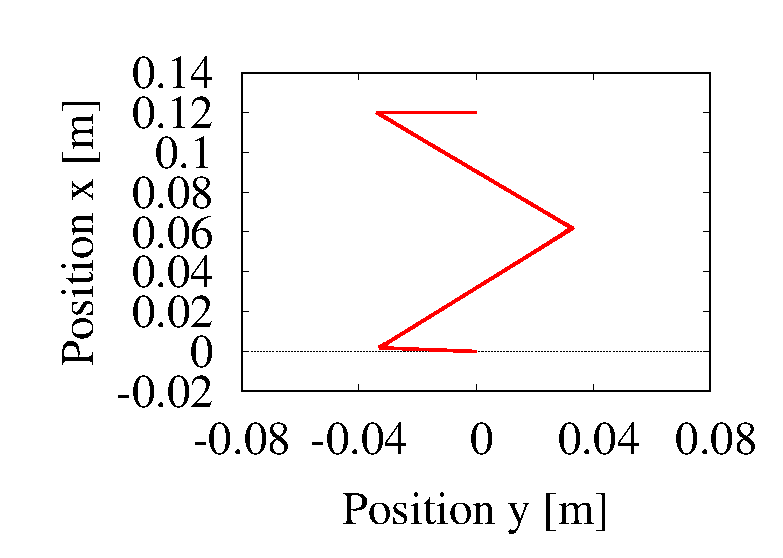
\includegraphics[width=1.0\linewidth]{./fig/CDSSpline.eps}
%     \footnotesize{\hspace{30pt}(a)}
%   \end{minipage}
%   \begin{minipage}{0.333\linewidth}
%     \centering
%     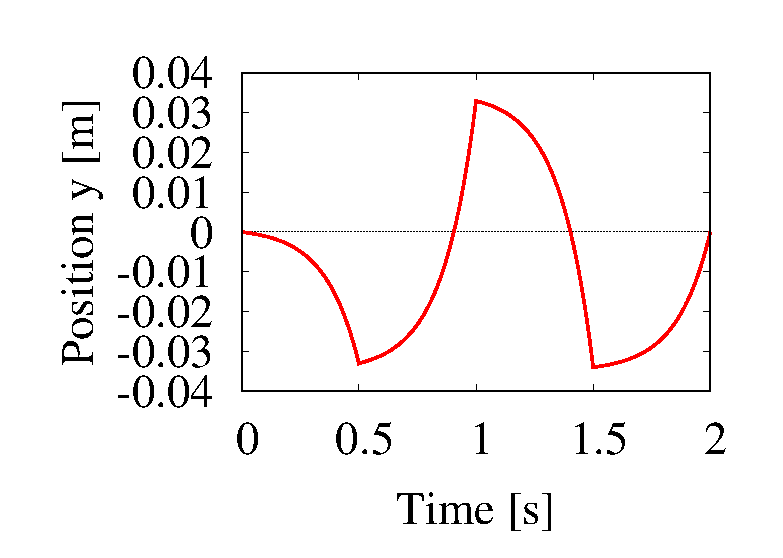
\includegraphics[width=1.0\linewidth]{./fig/CDSTimeY.eps}
%     \footnotesize{\hspace{30pt}(b)}
%   \end{minipage}
%   \begin{minipage}{0.333\linewidth}
%     \centering
%     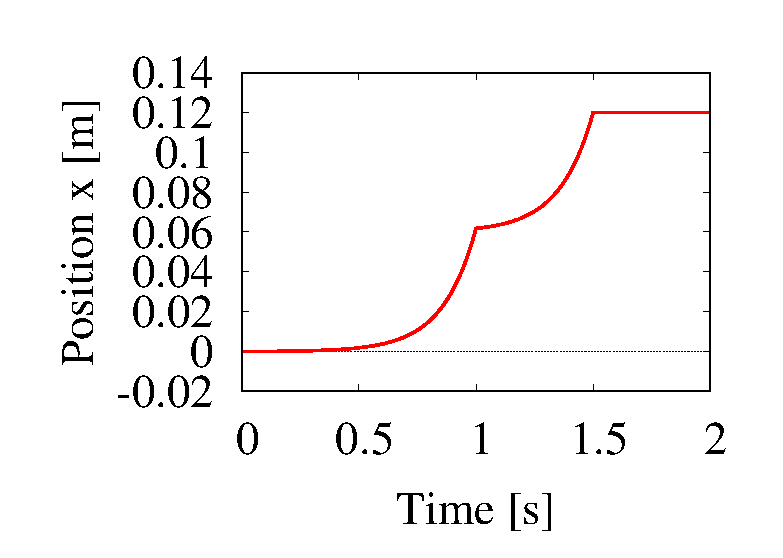
\includegraphics[width=1.0\linewidth]{./fig/CDSTimeX.eps}
%     \footnotesize{\hspace{30pt}(c)}
%   \end{minipage}
%   \caption{Simuration result of CDS.}
%   \label{fig:CDS}
% \end{figure}
\subsection{Cotinuous Heel-to-Toe Tajectories}
CDSでは,片脚支持期間において目標VRPが固定される.そのため,eCMPが固定されCoPの許容できる範囲が固定される% .両脚支持期間から片脚期間へ切り替える瞬間に,目標eCMPはつま先へ移動していることが望ましい.
そこで,CHTは遊脚動作によるモーメントを抑えるようにeCMPが移動するため許容範囲が広がり,より安定な歩行動作を可能とする.% そこで,各ステップでの目標着地位置$\bm{r}_f^{des,i}$からつま先およびかかとまでのオフセットを考慮して,以下のように各ステップでの目標VRPを決める.
% \begin{align}
% %#######################################################################
%   \bm{r}_{f,T}^{des,i}
%   &=\bm{r}_{f}^{des,i}
%     +\bm{R}_a^{des,i}
%     \begin{bmatrix}
%       \ob{{x}}_{vrp,T}&0&0
%     \end{bmatrix}^{T}\\
% %#######################################################################
% \bm{r}_{f,H}^{des,i}
%   &=\bm{r}_{f}^{des,i}
%     +\bm{R}_a^{des,i}
%     \begin{bmatrix}
%       \ob{{x}}_{vrp,H}&0&0
%     \end{bmatrix}^{T}
% \end{align}
% % ##########################################################################
% 式中の$\ob{{x}}_{vrp,T},~\ob{{x}}_{vrp,H}$はそれぞれ目標Toe--VRPオフセット,目標Heel--VRPオフセットと呼ぶ.また,$\bm{R}_{a}^{des,i}$は目標着地位置における目標の足の姿勢を表す.
% \begin{align}
% %#######################################################################
%   \bm{r}_{vrp,T}^{des,i}
%   &=\bm{r}_{f,T}^{des,i}
%     +\bm{R}_a^{des,i}
%     \begin{bmatrix}
%       0&0&\ob{{z}}_{vrp}
%     \end{bmatrix}^{T}\\
% %#######################################################################
%   \bm{r}_{vrp,H}^{des,i}
%   &=\bm{r}_{f,H}^{des,i}
%     +\bm{R}_a^{des,i}
%     \begin{bmatrix}
%       0&0&\ob{{z}}_{vrp}
%     \end{bmatrix}^{T}
% \end{align}
% % ##########################################################################
% 同様にして,目標のDCMの軌道を算出できる.よって各ステップでの目標VRPは以上で定義される.
% さらに,
% まず,各ステップでの目標VRPから各ステップのそれぞれ目標DCMを決定する.
\begin{align}
\bm{r}_{X,TH^{init}}^{des,i}
  &=\bm{r}_{vrp,T}^{des,i}
  +e^{-\frac{T_{TH}}{T_X}}(\bm{r}_{X,HT^{init}}^{des,i+1}-\bm{r}_{vrp,T}^{des,i})\nonumber\\
  % #######################################################################
 \bm{r}_{X,HT^{init}}^{des,i}
  &=\bm{r}_{vrp,H}^{des,i}
  +e^{-\frac{T_{HT}}{T_X}}(\bm{r}_{X,TH^{init}}^{des,i+1}-\bm{r}_{vrp,H}^{des,i})\nonumber\\
   % \label{eq:cht1}
%\end{align}
%式中の$T_{TH}$=$(1-\alpha_{HT})T_{step}$であり,$T_{HT}$=$\alpha_{HT}T_{step}$である.
%\begin{align}
%#######################################################################
  \bm{r}_{X,DS^{init}}^{des,i}
  &=\bm{r}_{vrp,T}^{des,i-1}
  +e^{-\frac{T_{DS}^{init}}{T_X}}(\bm{r}_{X,HT^{init}}^{des,i}-\bm{r}_{vrp,T}^{des,i-1})\nonumber\\
%#######################################################################
  \bm{r}_{X,DS^{end}}^{des,i}
  &=\bm{r}_{vrp,H}^{des,i}
    +e^{\frac{T_{DS}^{end}}{T_X}}(\bm{r}_{X,HT^{init}}^{des,i}-\bm{r}_{vrp,H}^{des,i})\nonumber
%#######################################################################
%   \dot{\bm{r}}_{X,DS^{init}}^{des,i}
%   &=\frac{1}{T_X}(\bm{r}_{X,DS^{init}}^{des}-\bm{r}_{vrp,T}^{des,i-1})\\
%   % #######################################################################
%   \dot{\bm{r}}_{X,DS^{end}}^{des,i}
%   &=\frac{1}{T_X}(\bm{r}_{X,DS^{end}}^{des}-\bm{r}_{vrp,H}^{des,i})\\
% %#######################################################################
%   \ddot{\bm{r}}_{X,DS^{init}}^{des,i}
%   &= \frac{1}{T_X^2}
%     e^{-\frac{T_{DS}^{init}}{T_X}}(\bm{r}_{X,HT^{init}}^{des,i}-\bm{r}_{vrp,T}^{des,i-1})\\
% %#######################################################################
%   \ddot{\bm{r}}_{X,DS^{end}}^{des,i}
%   &=\frac{1}{T_X^2}
%     e^{\frac{T_{DS}^{end}}{T_X}}(\bm{r}_{X,HT^{init}}^{des,i}-\bm{r}_{vrp,H}^{des,i})
\end{align}
式中,$T_{TH}$=$(1-\alpha_{HT})T_{step}$であり,$T_{HT}$=$\alpha_{HT}T_{step}$である.
\begin{figure}[b]
\begin{minipage}{0.333\hsize}
        \hspace{2mm}
      \end{minipage}
  \begin{minipage}{0.2\linewidth}
    \centering
    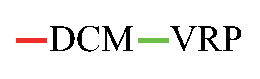
\includegraphics[width=1.0\linewidth]{./fig/key2.eps}
  \end{minipage}
   \begin{minipage}{0.333\hsize}
        \hspace{2mm}
      \end{minipage}
    
  \begin{minipage}{0.48\linewidth}
    \centering
    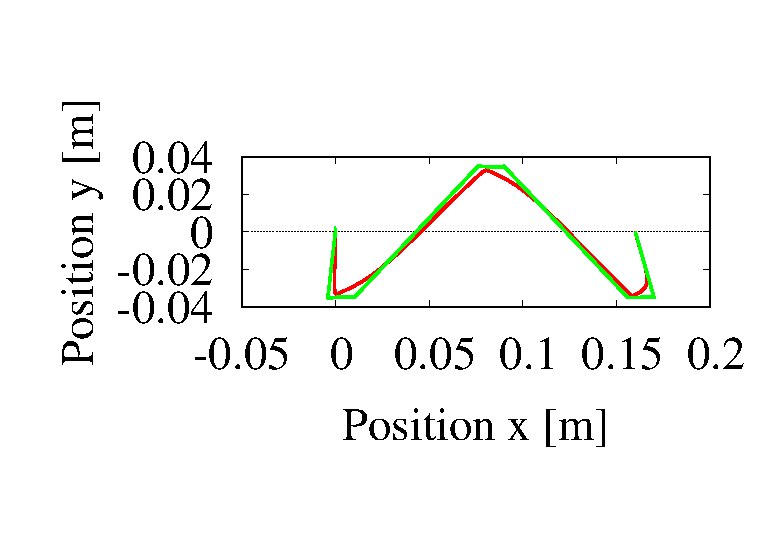
\includegraphics[width=1.0\linewidth]{./fig/Position1.eps}
    \footnotesize{\hspace{30pt}(a)}
  \end{minipage}
  \begin{minipage}{0.48\linewidth}
    \centering
    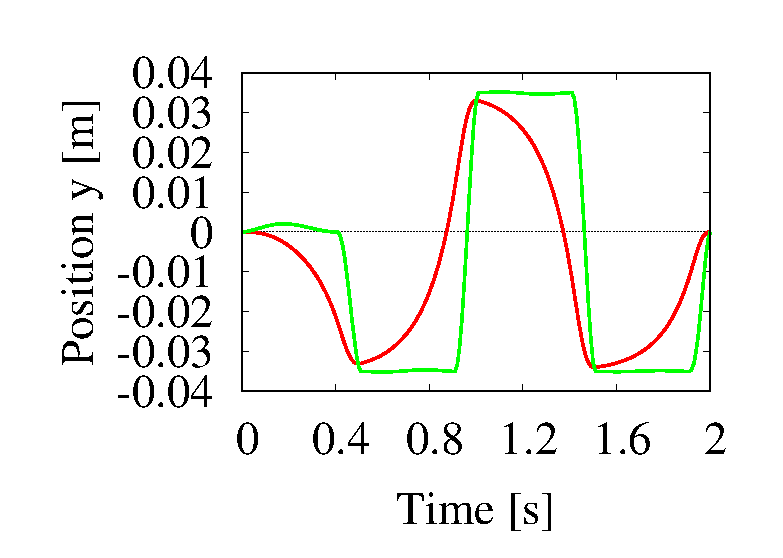
\includegraphics[width=1.0\linewidth]{./fig/rXKIDOU.eps}
    \footnotesize{\hspace{30pt}(b)}
  \end{minipage}
  % \begin{minipage}{0.32\linewidth}
  %   \centering
  %   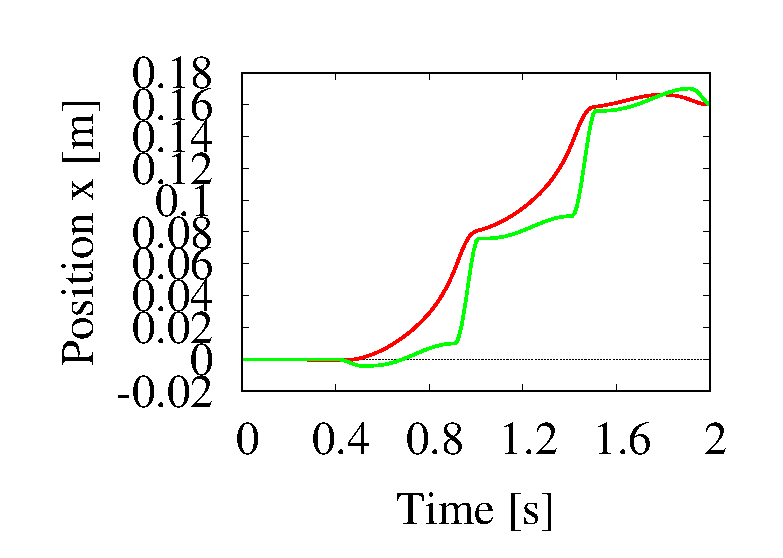
\includegraphics[width=1.0\linewidth]{./fig/HTkidou.eps}
  %   \footnotesize{\hspace{30pt}(c)}
  % \end{minipage}
  \caption{Simuration result of CHT.}
  \label{fig:CHT}
\end{figure}
両脚支持期間の開始時と終了時におけるDCMの目標位置は以上で定義され,速度および加速度は時間微分により求まる.また,CHTでは,片脚支持期間における軌道および両脚支持期間における軌道が上記を境界値とする多項式補間によって決定される
\subsection{軌道生成シミュレーション}
% CHTでは,片脚支持期間における軌道および両脚支持期間における軌道が上記を境界値とする多項式補間によって決定される.
% \bal[CHT1]{
%   \bm{r}_{vrp,T}^{des,0}
%   =\frac{1}{1-e^{-\frac{T_{TH}}{T_X}}}\bm{r}_C(0)
%   +\frac{1}{1-e^{\frac{T_{TH}}{T_X}}}\bm{r}_{X,HT^{init}}^{des,1}
% }
% また,CDSと同様に初期の目標VRPは以上で定義される
今回は歩幅を8 cmとし,2秒間で二歩踏み出す軌道生成を行った.Fig.~\ref{fig:CHT}には,DCMおよびVRPの位置を示した.
VRPが連続的に移動していることがわかった.また,定めた値に正しくDCMを制御できた.
% \begin{figure}[h]
% \begin{minipage}{0.333\hsize}
%         \hspace{2mm}
%       \end{minipage}
%   \begin{minipage}{0.2\linewidth}
%     \centering
%     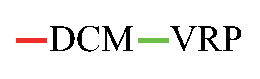
\includegraphics[width=1.0\linewidth]{./fig/key2.eps}
%   \end{minipage}
%    \begin{minipage}{0.333\hsize}
%         \hspace{2mm}
%       \end{minipage}
    
%   \begin{minipage}{0.48\linewidth}
%     \centering
%     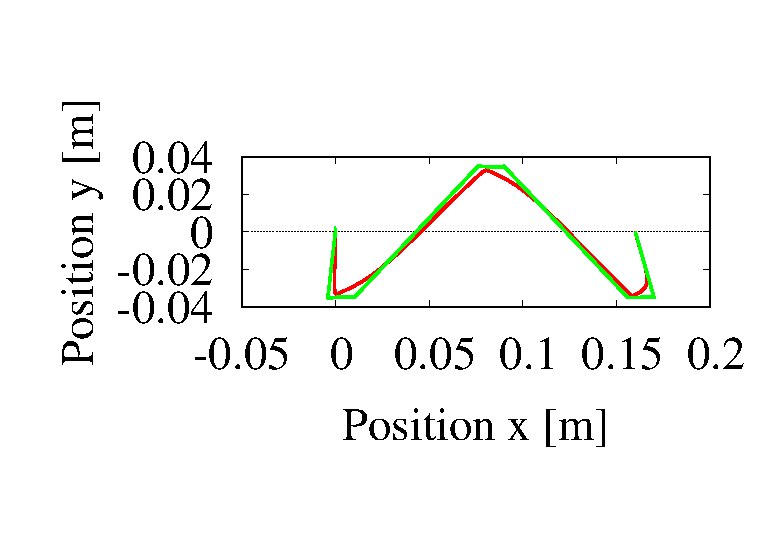
\includegraphics[width=1.0\linewidth]{./fig/Position1.eps}
%     \footnotesize{\hspace{30pt}(a)}
%   \end{minipage}
%   \begin{minipage}{0.48\linewidth}
%     \centering
%     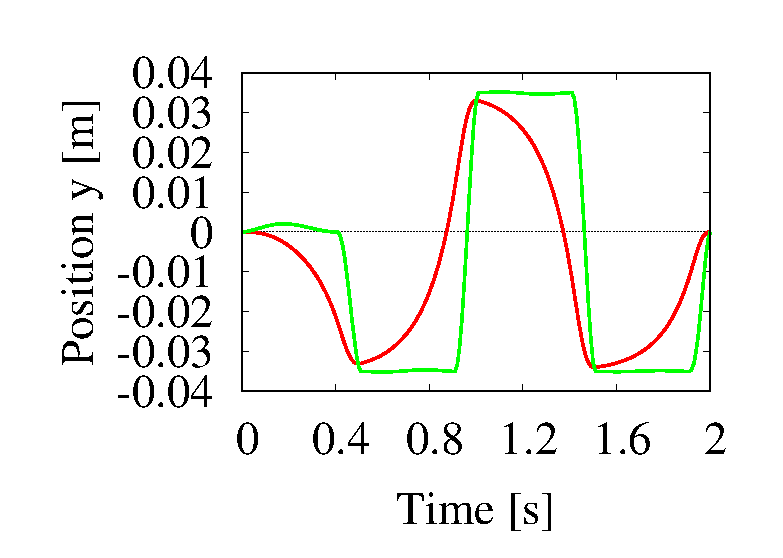
\includegraphics[width=1.0\linewidth]{./fig/rXKIDOU.eps}
%     \footnotesize{\hspace{30pt}(b)}
%   \end{minipage}
%   % \begin{minipage}{0.32\linewidth}
%   %   \centering
%   %   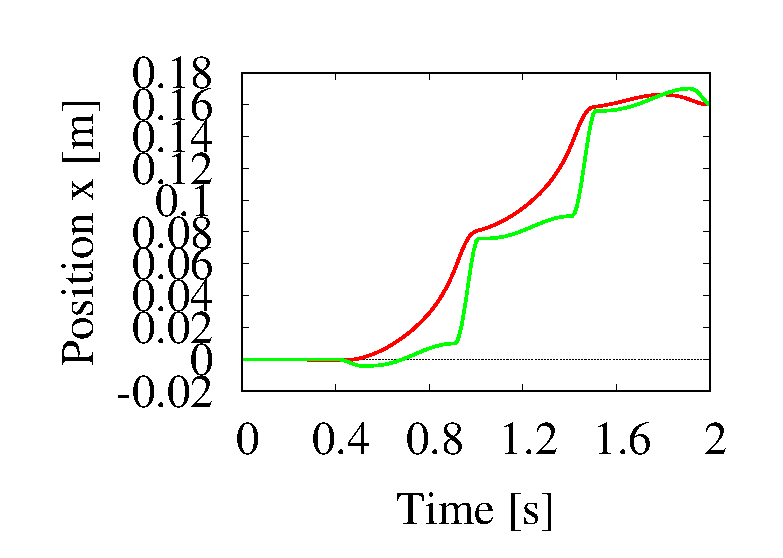
\includegraphics[width=1.0\linewidth]{./fig/HTkidou.eps}
%   %   \footnotesize{\hspace{30pt}(c)}
%   % \end{minipage}
%   \caption{Simuration result of CHT.}
%   \label{fig:CHT}
% \end{figure}
%#############################################################
\section{歩行におけるトルク比較}
\subsection{先行研究における歩行}
先行研究でのCHTによるシミュレーション歩行において,歩幅を8 cmとし$T_{DS}$および$T_{SS}$をそれぞれ0.1 s,0.4 sとした際の脚部の関節トルクが許容トルクである4.5 Nmであった.ここで,$T_{DS}$は両脚支持期間の時間を表し,$T_{SS}$は片脚支持期間である.左右の最大トルクは一緒であるため,今回は右脚関節に着目しトルクの検証を行った.以上の条件での右脚におけるトルクをFig.~\ref{fig:CHT1}(a)に示した.2.25 s時点の片脚支持期間において,Joint4(右膝関節)の瞬時の許容トルクである4.5 Nmに達していることがわかる.実機実装を行うためには,少なくとも片脚支持期間におけるトルクを小さくする必要がある.そこで,シミュレーション環境にて,トルクを下げる方法を以下に示した.右膝関節の最大トルクを$\tau_{4,\rm{max}}$と表す.
% ==============================================
% \begin{table}[b]
%   \centering
%   \caption{Joint allowable torques.}
%   \vspace{-2mm}
%   \begin{tabular}[t]{|c||c|c|c|c|c|c|}
%     \hline
%     Joint number & 1 & 2 & 3 & 4 & 5 & 6\\ \hline\hline
%     Regular use [Nm]& 1.5 & 2.0 & 1.5 & 2.0 & 1.5 & 1.5\\ \hline
%     Instantaneous [Nm]& 3.0& 4.5 & 3.0 & 4.5 & 3.0 & 3.0\\ \hline
%   \end{tabular}
%   \label{tab:table1}
% \end{table}
% #####################################################################
% \begin{figure}[h]
% \begin{minipage}{0.4\hsize}
%         \hspace{2mm}
%       \end{minipage}
%   \begin{minipage}{0.15\linewidth}
%     \centering
%     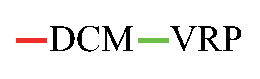
\includegraphics[width=1.0\linewidth]{./fig/key2.eps}
%   \end{minipage}
%    \begin{minipage}{0.333\hsize}
%         \hspace{2mm}
%       \end{minipage}
    
%   \begin{minipage}{0.48\linewidth}
%     \centering
%     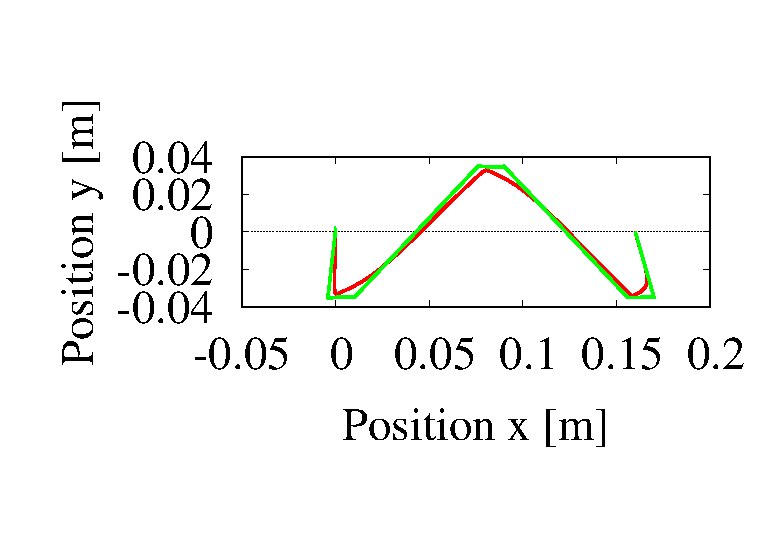
\includegraphics[width=1.0\linewidth]{./fig/Position1.eps}
%     \footnotesize{\hspace{30pt}(a)}
%   \end{minipage}
%   \begin{minipage}{0.48\linewidth}
%     \centering
%     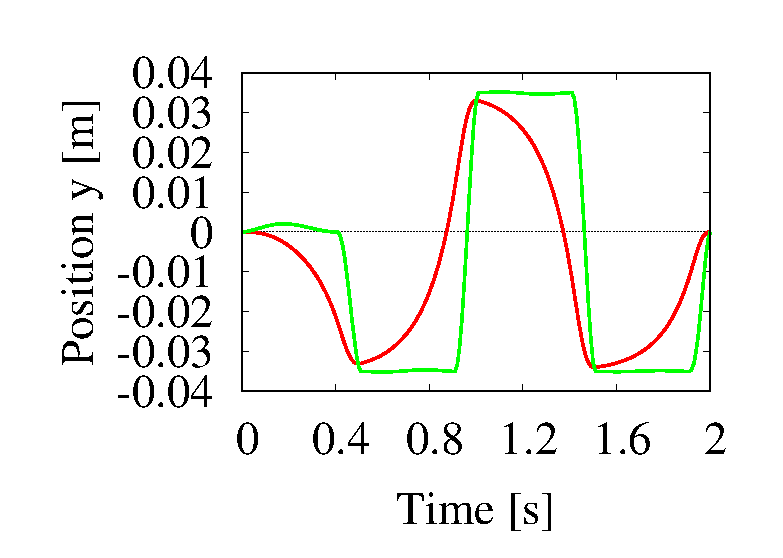
\includegraphics[width=1.0\linewidth]{./fig/rXKIDOU.eps}
%     \footnotesize{\hspace{30pt}(b)}
%   \end{minipage}
%   % \begin{minipage}{0.32\linewidth}
%   %   \centering
%   %   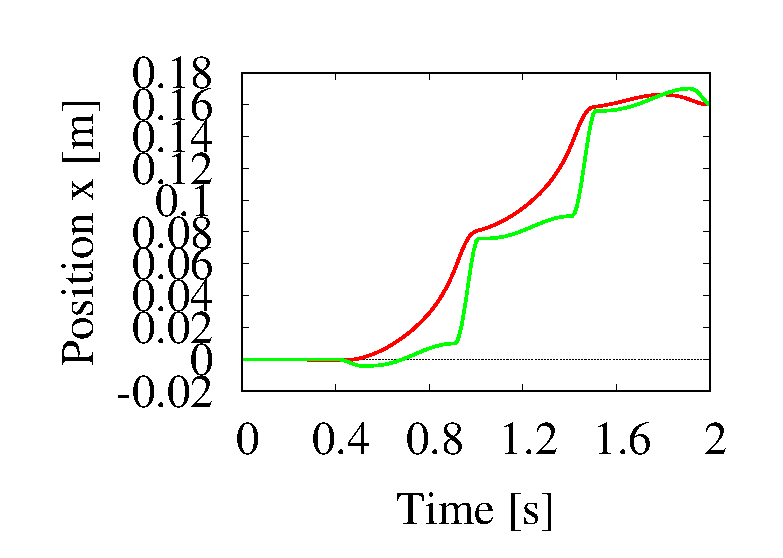
\includegraphics[width=1.0\linewidth]{./fig/HTkidou.eps}
%   %   \footnotesize{\hspace{30pt}(c)}
%   % \end{minipage}
%   \caption{Simuration result of CHT.}
%   \label{fig:CHT}
% \end{figure}
%#####################################################################
% \begin{figure}[b]
%   \begin{minipage}{0.5\linewidth}
%     \centering
%     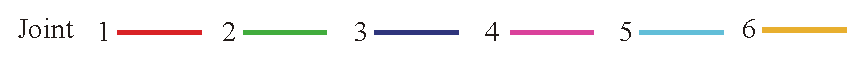
\includegraphics[width=1.0\linewidth]{./fig/key6leg.eps}
%   \end{minipage}
%   \begin{minipage}{0.48\linewidth}
%     \centering
%     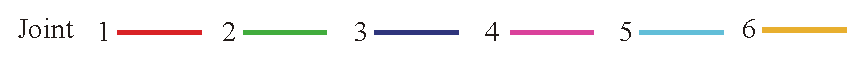
\includegraphics[width=1.0\linewidth]{./fig/key6leg.eps}
%   \end{minipage}
%   \begin{minipage}{0.48\linewidth}
%     \centering
%     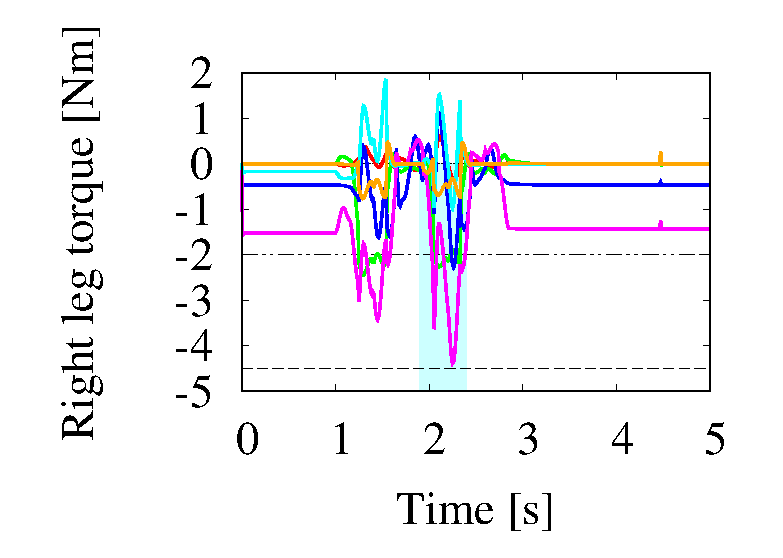
\includegraphics[width=1.0\linewidth]{./fig/original.eps}
%   \end{minipage}
%    \begin{minipage}{0.49\linewidth}
%     \centering
%     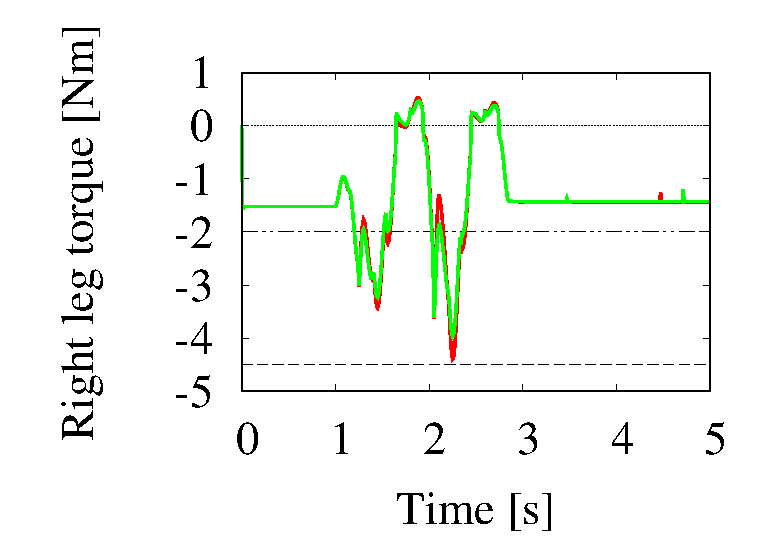
\includegraphics[width=1.0\linewidth]{./fig/hohaba.eps}
%   \end{minipage}
%    \begin{minipage}{0.48\linewidth}
%     \centering
%     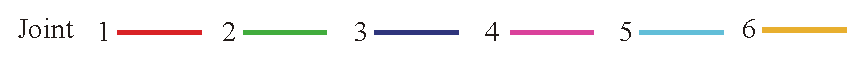
\includegraphics[width=1.0\linewidth]{./fig/key6leg.eps}
%   \end{minipage}
%   \begin{minipage}{0.48\linewidth}
%     \centering
%     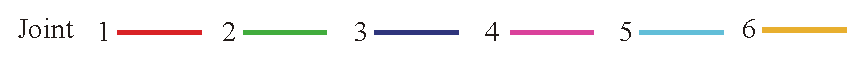
\includegraphics[width=1.0\linewidth]{./fig/key6leg.eps}
%   \end{minipage}
%   \begin{minipage}{0.49\linewidth}
%     \centering
%     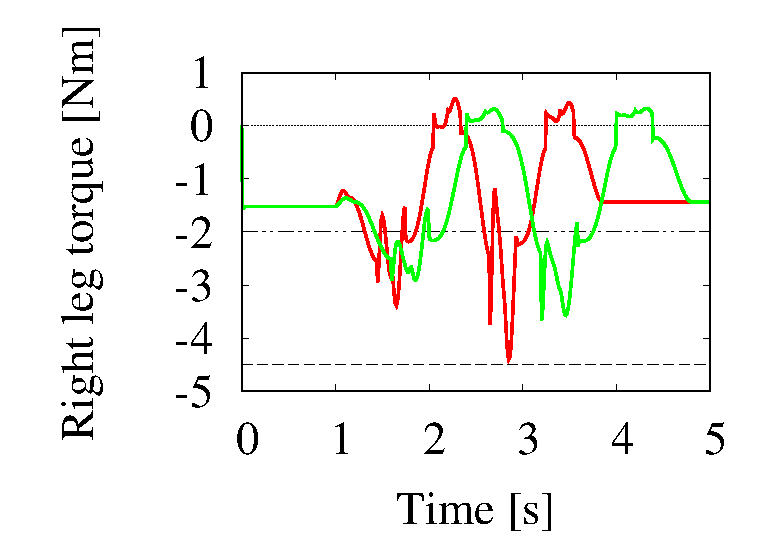
\includegraphics[width=1.0\linewidth]{./fig/TDS.eps}
%   \end{minipage}
%    \begin{minipage}{0.49\linewidth}
%     \centering
%     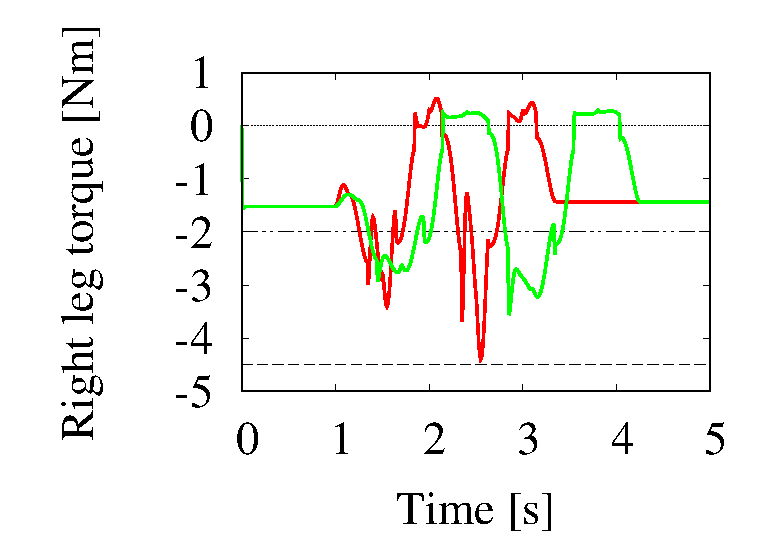
\includegraphics[width=1.0\linewidth]{./fig/TSS.eps}
%   \end{minipage}
%   \caption{Simuration result of torque.}
%   \label{fig:CHT1}
% \end{figure}

 % ############################################################################
\subsection{$T_{step}$における比較}
$T_{DS}$および$T_{SS}$の時間比は1:1とし,$T_{step}$を0.1 sずつ増加させトルクの比較を行った.Table~\ref{tab:table2}にはシミュレーション条件を示した.Fig.~\ref{fig:CHT1}(b)より$T_{step}$が0.6 sの際のトルクは-4.50 Nmであり,$T_{step}$が0.8 sの際のトルクは-3.72 Nmと,$T_{step}$が長い程トルクが小さくなることがわかる.
% ==============================================
% \begin{table}[b]
%   \centering
%   \caption{Step period.}
%   \vspace{-2mm}
%   \begin{tabular}[t]{|c||c|c|c|}
%     \hline
%     $Tstep$ [s]& 0.6 & 0.7 & 0.8 \\ \hline
%     $T_{DS}$ [s]& 0.3 & 0.35 & 0.4 \\ \hline
%     $T_{SS}$ [s]& 0.3 & 0.35 & 0.4 \\ \hline
%     $\tau_{4,\rm{max}}$ [Nm] & -4.50 & -4.07 & -3.72 \\\hline
%   \end{tabular}
%   \label{tab:table2}
% \end{table}
%###############################################################
% \begin{figure}[h]
%   \begin{minipage}{0.333\linewidth}
%     \centering
%     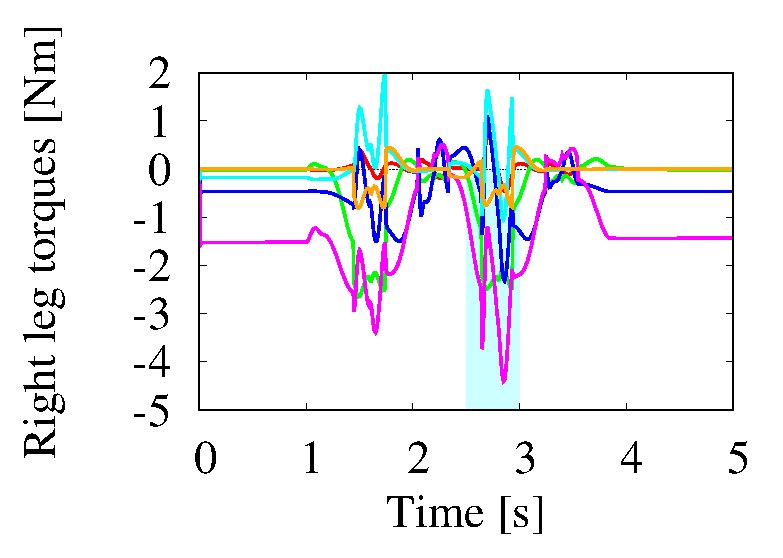
\includegraphics[width=1.0\linewidth]{./fig/0505.eps}
%     \footnotesize{\hspace{30pt}(a)}
%   \end{minipage}
%   \begin{minipage}{0.333\linewidth}
%     \centering
%     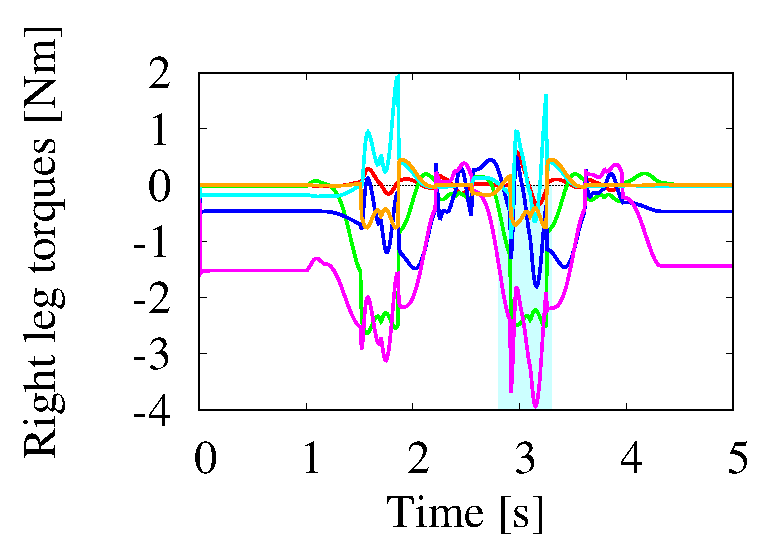
\includegraphics[width=1.0\linewidth]{./fig/0521.eps}
%     \footnotesize{\hspace{30pt}(b)}
%   \end{minipage}
%   \begin{minipage}{0.333\linewidth}
%     \centering
%     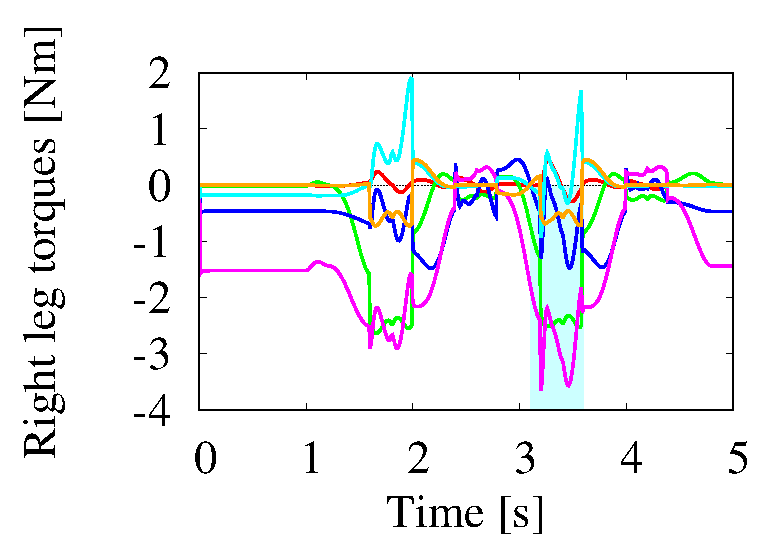
\includegraphics[width=1.0\linewidth]{./fig/0522.eps}
%     \footnotesize{\hspace{30pt}(c)}
%   \end{minipage}
%   \caption{Simuration result of torque.}
%   \label{fig:CHT2}
% \end{figure}

% #############################################################################
% \subsection{$T_{DS}$における比較}
% $T_{SS}$は0.3 sとし,$T_{DS}$を0.1 sずつ増加させることによりトルクの比較を行った.Fig.\ref{fig:CHT3}より$T_{DS}$によるトルクの変動はあまり見られないことがわかる.
% % ############################################################################
% \begin{table}[h]
%   \centering
%   \caption{Step period.}
%   \vspace{-3mm}
%   \begin{tabular}[t]{|c||c|c|c|}
%     \hline
%     $Tstep$ [s]& 0.4 & 0.5 & 0.6 \\ \hline
%     $T_{DS}$ [s]& 0.1 & 0.2 & 0.3 \\ \hline
%    $T_{SS}$ [s]& 0.3 & 0.3 & 0.3 \\ \hline
%    $\tau_{4,\rm{max}}$ [Nm] & -4.51 & -4.49 & -4.50 \\\hline
%   \end{tabular}
%   \label{tab:table3}
% \end{table}

% \begin{figure}[h]
%   \begin{minipage}{0.333\linewidth}
%     \centering
%     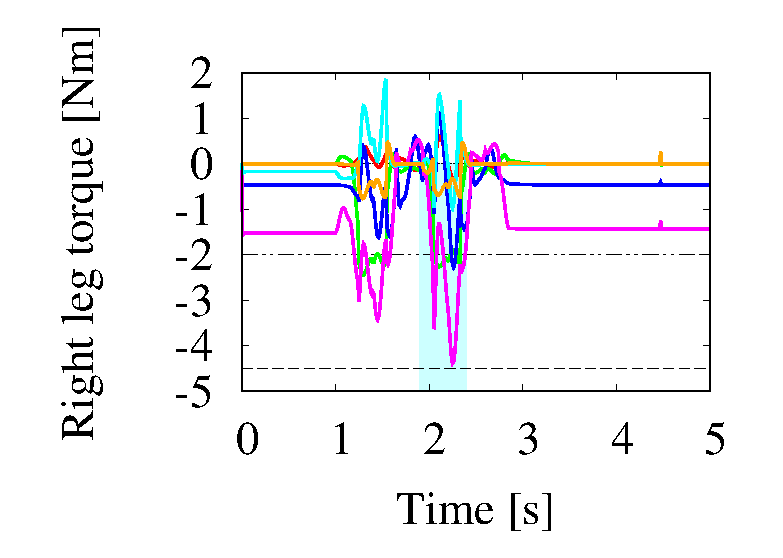
\includegraphics[width=1.0\linewidth]{./fig/original.eps}
%     \footnotesize{\hspace{30pt}(a)}
%   \end{minipage}
%   \begin{minipage}{0.333\linewidth}
%     \centering
%     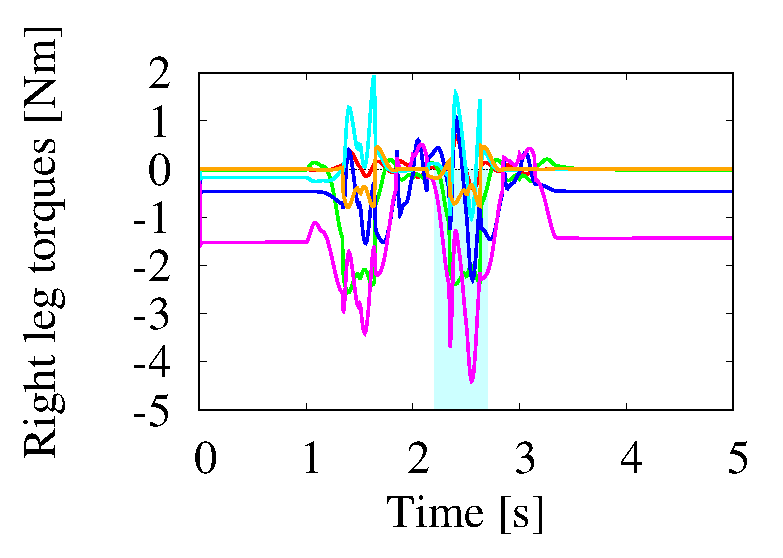
\includegraphics[width=1.0\linewidth]{./fig/0504.eps}
%     \footnotesize{\hspace{30pt}(b)}
%   \end{minipage}
%   \begin{minipage}{0.333\linewidth}
%     \centering
%     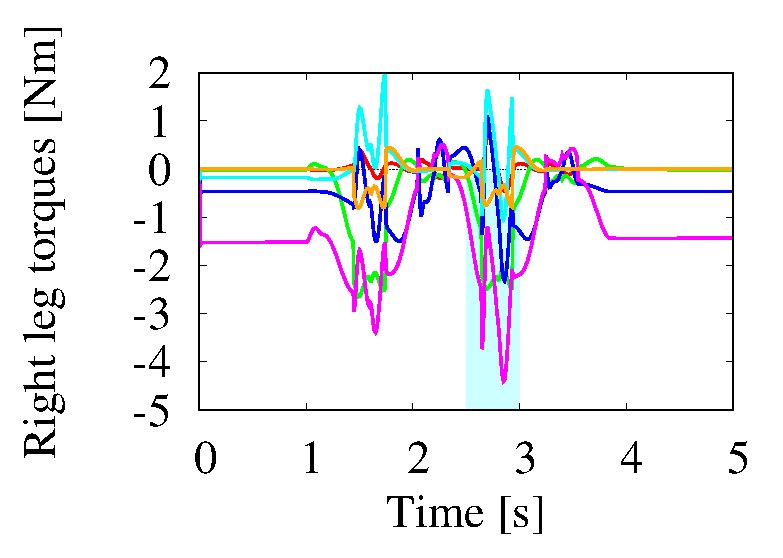
\includegraphics[width=1.0\linewidth]{./fig/0505.eps}
%     \footnotesize{\hspace{30pt}(c)}
%   \end{minipage}
%   \caption{Simuration result of torque.}
%   \label{fig:CHT3}
% \end{figure}
% ############################################################################
\subsection{$T_{SS}$における比較}
$T_{DS}$は0.2 sとし,$T_{SS}$を増加させることによりトルクの比較を行った.Table~\ref{tab:table4}にはシミュレーション条件を示した.Fig.~\ref{fig:CHT1}(c)より$T_{SS}$が0.3 sの際のトルクは-4.50 Nmであり,$T_{SS}$が0.5 sの際のトルクは-3.55 Nmと,$T_{SS}$が長い程トルクが小さくなることがわかる.
%##########################################################
% \begin{table}[b]
%   \centering
%   \caption{Step period.}
%   \vspace{-2mm}
%   \begin{tabular}[t]{|c||c|c|c|}
%     \hline
%     $Tstep$ [s]& 0.5 & 0.6 & 0.7 \\ \hline
%     $T_{DS}$ [s]& 0.2 & 0.2 & 0.2 \\ \hline
%    $T_{SS}$ [s]& 0.3 & 0.4 & 0.5 \\ \hline
%    $\tau_{4,\rm{max}}$ [Nm] & -4.49 & -3.64 & -3.55 \\\hline
%   \end{tabular}
%   \label{tab:table4}
% \end{table}
%##################################################################
% \begin{figure}[h]
%   \begin{minipage}{0.333\linewidth}
%     \centering
%     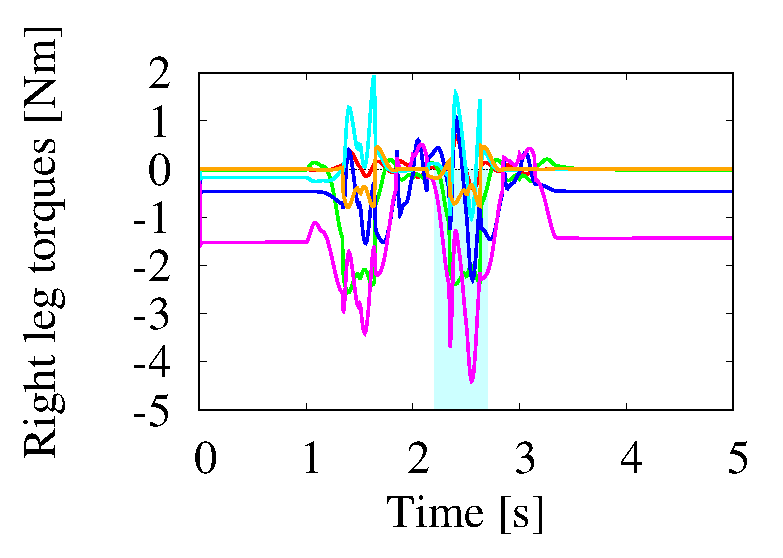
\includegraphics[width=1.0\linewidth]{./fig/0504.eps}
%     \footnotesize{\hspace{30pt}(a)}
%   \end{minipage}
%   \begin{minipage}{0.333\linewidth}
%     \centering
%     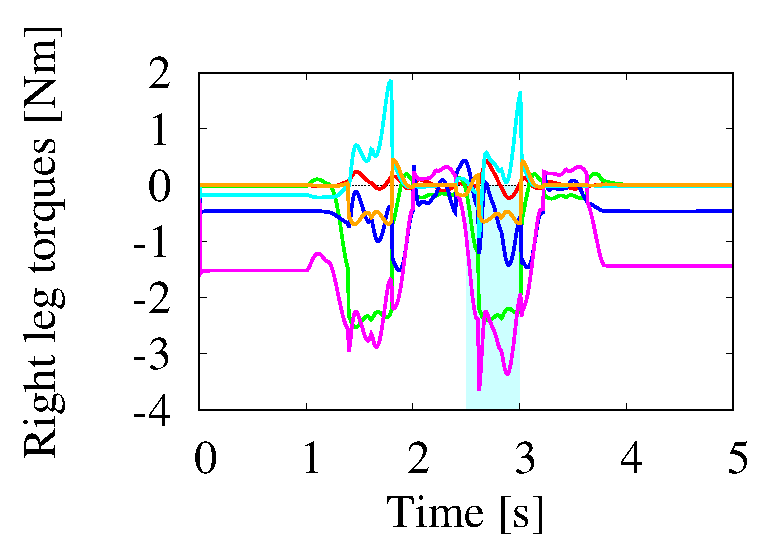
\includegraphics[width=1.0\linewidth]{./fig/0506.eps}
%     \footnotesize{\hspace{30pt}(b)}
%   \end{minipage}
%   \begin{minipage}{0.333\linewidth}
%     \centering
%     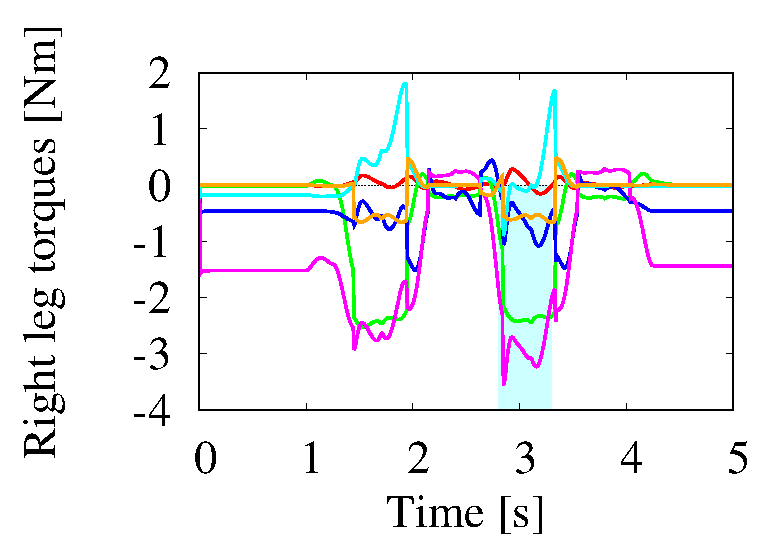
\includegraphics[width=1.0\linewidth]{./fig/0510.eps}
%     \footnotesize{\hspace{30pt}(c)}
%   \end{minipage}
%   \caption{Simuration result of torque.}
%   \label{fig:CHT4}
% \end{figure}

% #############################################################################
\subsection{歩幅における比較}
$T_{step}$を0.4 s,$T_{DS}$を0.1 s,$T_{SS}$を0.3 sとした際,ステップ周期を変化させずに,歩幅によるトルクの比較を行った.Table~\ref{tab:table5}にはシミュレーション条件を示した.Fig.~\ref{fig:CHT1}(d)より,歩幅が0.08 mの際のトルクは-4.49 Nmであり,歩幅が0.06 mの際のトルクは-4.04 Nmと,歩幅を小さくすることでトルクを抑えることが可能であることがわかる.
   %    以上のことを元にして,動歩行が可能であるパラメータを見つけるとともに,トルクの検証を行う.
% ############################################################################
% \begin{table}[b]
%   \centering
%   \caption{Strides for comparison in strides.}
%   \vspace{-2mm}
%   \begin{tabular}[t]{|c||c|c|c|}
%     \hline
%   stride [m]& 0.08 & 0.07 & 0.06 \\\hline 
%    $\tau_{4,\rm{max}}$ [Nm] & -4.50 & -4.28 & -4.04 \\\hline
%   \end{tabular}
%   \label{tab:table5}
% \end{table}
%#######################################################################
% \begin{figure}[h]
%   \begin{minipage}{0.333\linewidth}
%     \centering
%     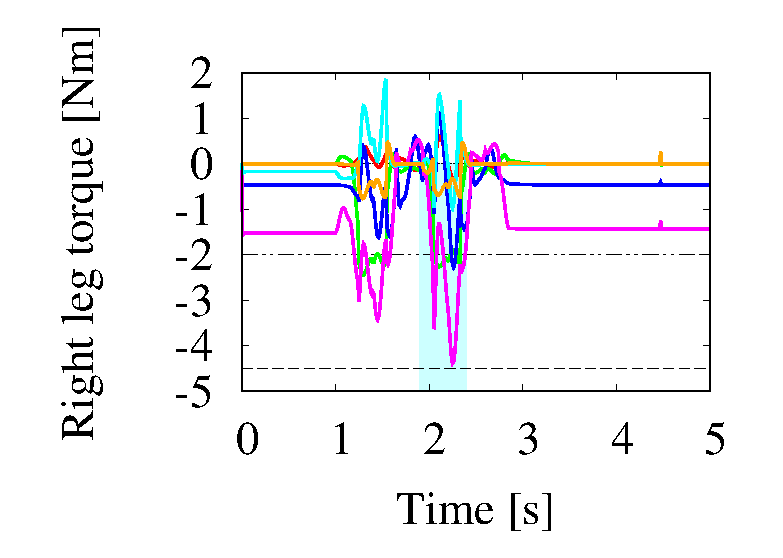
\includegraphics[width=1.0\linewidth]{./fig/original.eps}
%     \footnotesize{\hspace{30pt}(a)}
%   \end{minipage}
%   \begin{minipage}{0.333\linewidth}
%     \centering
%     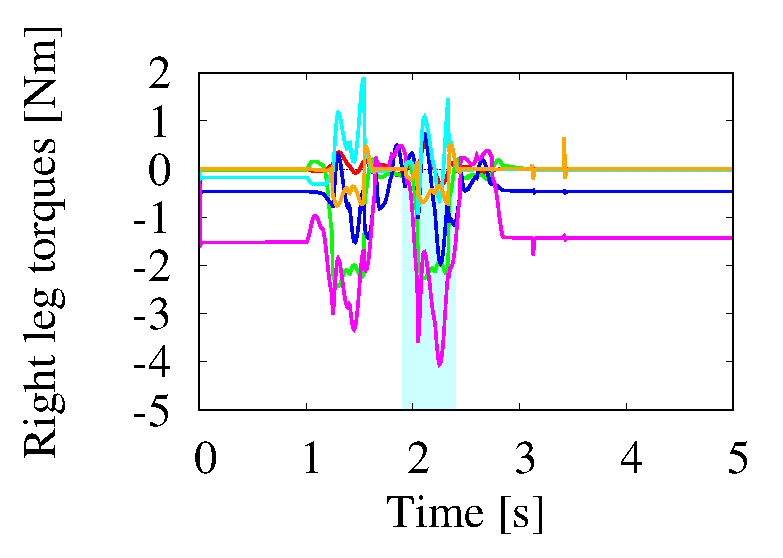
\includegraphics[width=1.0\linewidth]{./fig/0507.eps}
%     \footnotesize{\hspace{30pt}(b)}
%   \end{minipage}
%   \begin{minipage}{0.333\linewidth}
%     \centering
%     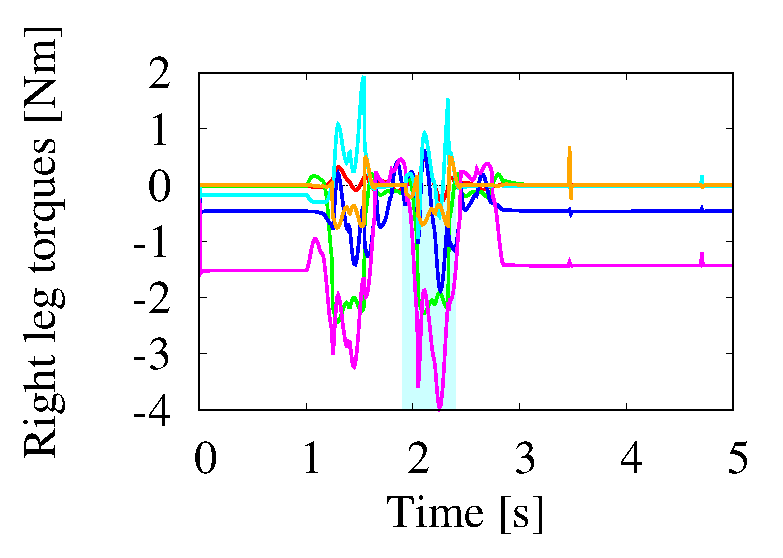
\includegraphics[width=1.0\linewidth]{./fig/0508.eps}
%     \footnotesize{\hspace{30pt}(c)}
%   \end{minipage}
%   \caption{Simuration result of torque.}
%   \label{fig:CHT5}
% \end{figure}
%#############################################################################
% \newpage\subsection{$\alpha_{DS}$および$\alpha_{HT}$における比較}
% $\alpha_{DS}$を変化させた際と$\alpha_{HT}$を変化させた際でそれぞれ比較を行った.Fig.\ref{fig:CHT6}より$\alpha_{DS}$および$\alpha_{HT}$を変化させた場合,トルクにおいて変化は見られなかった.
% % ############################################################################
% \begin{table}[h]
%   \centering
%   \caption{Step period and alpha.}
%   \vspace{-3mm}
%   \begin{tabular}[t]{|c||c|c|c|}
%     \hline
%     $Tstep$ [s]& 0.4 & 0.4 & 0.4 \\ \hline
%     $T_{DS}$ [s]& 0.1 & 0.1 & 0.1 \\ \hline
%     $T_{SS}$ [s]& 0.3 & 0.3 & 0.3 \\ \hline
%     $\alpha{DS}$ & 0.5 & 0.4 & 5.0 \\\hline
%     $\alpha_{HT}$ & 0.5 & 0.5 & 0.42 \\\hline
%    $\tau_{4,\rm{max}}$ [Nm] & -4.50 & -4.52 & -4.45 \\\hline
%   \end{tabular}
%   \label{tab:table6}
% \end{table}
% \begin{figure}[h]
%   \begin{minipage}{0.333\linewidth}
%     \centering
%     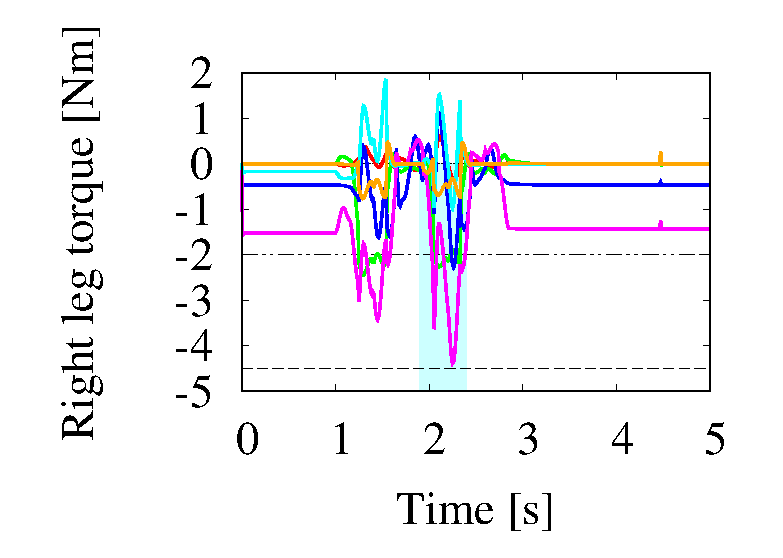
\includegraphics[width=1.0\linewidth]{./fig/original.eps}
%     \footnotesize{\hspace{30pt}(a)}
%   \end{minipage}
%   \begin{minipage}{0.333\linewidth}
%     \centering
%     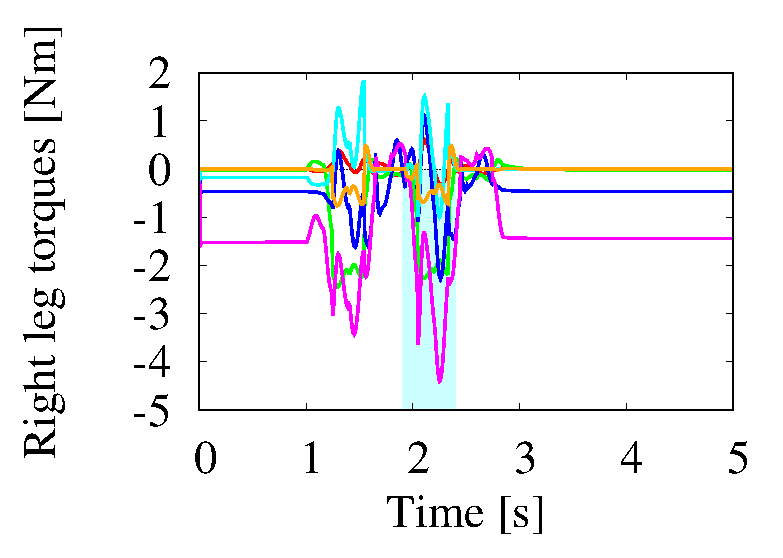
\includegraphics[width=1.0\linewidth]{./fig/0519.eps}
%     \footnotesize{\hspace{30pt}(b)}
%   \end{minipage}
%   \begin{minipage}{0.333\linewidth}
%     \centering
%     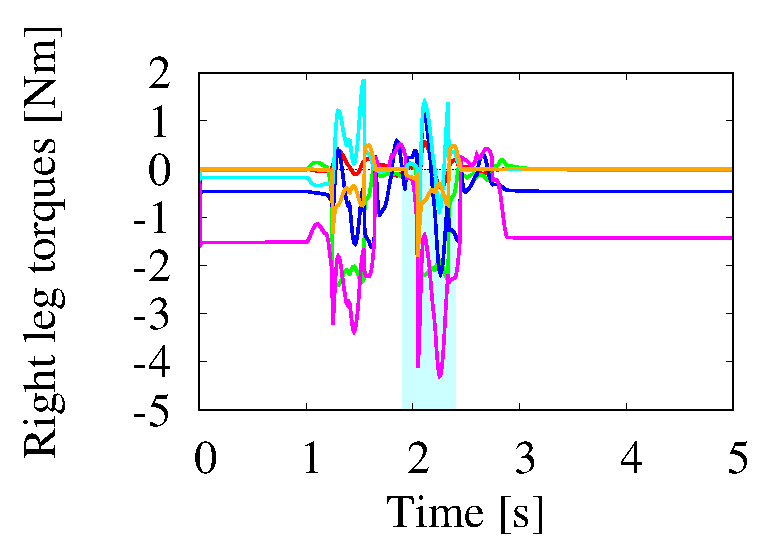
\includegraphics[width=1.0\linewidth]{./fig/0520.eps}
%     \footnotesize{\hspace{30pt}(c)}
%   \end{minipage}
%   \caption{Simuration result of torque.}
%   \label{fig:CHT6}
% \end{figure}
%
% #############################################################################
%
% ############################################################################
% \begin{figure}[h]
%   \begin{minipage}{0.333\linewidth}
%     \centering
%     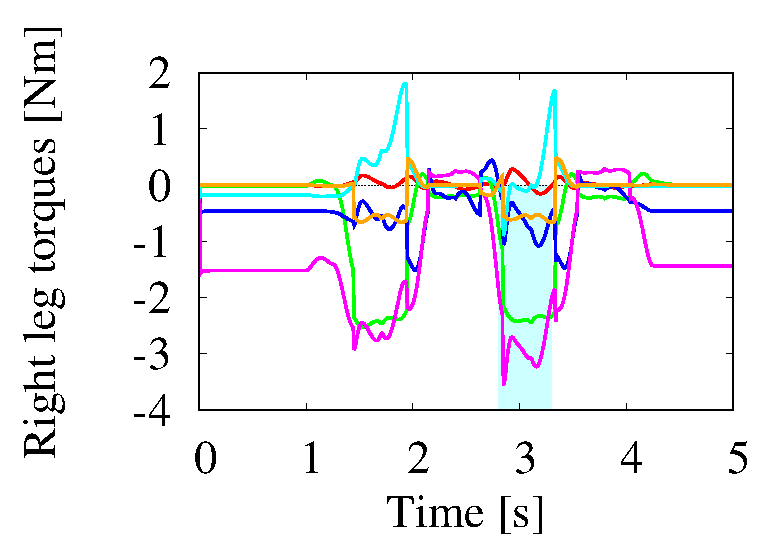
\includegraphics[width=1.0\linewidth]{./fig/0510.eps}
%     \footnotesize{\hspace{30pt}(a)}
%   \end{minipage}
%   \begin{minipage}{0.333\linewidth}
%     \centering
%     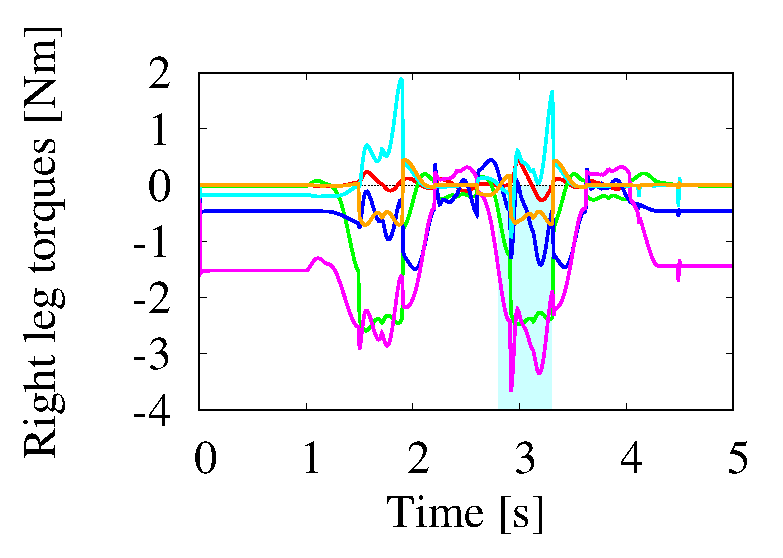
\includegraphics[width=1.0\linewidth]{./fig/0509.eps}
%     \footnotesize{\hspace{30pt}(b)}
%   \end{minipage}
%   \begin{minipage}{0.333\linewidth}
%     \centering
%     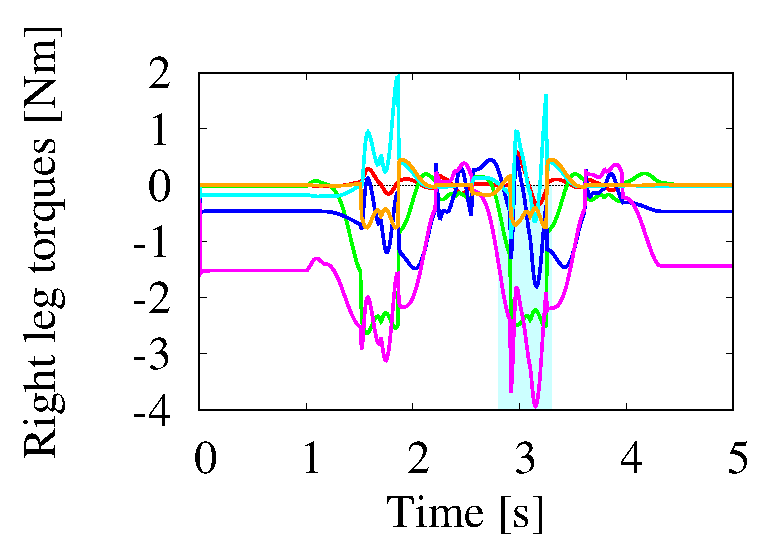
\includegraphics[width=1.0\linewidth]{./fig/0521.eps}
%     \footnotesize{\hspace{30pt}(c)}
%   \end{minipage}
%   \caption{Simuration result of CHT.}
%   \label{fig:CHT6}
% \end{figure}

%#############################################################################
% \subsection{VRPオフセットによる比較}
% 足首からのオフセットを変化させた際のトルクの比較を行った.Fig.\ref{fig:CHT7}およびFig.\ref{fig:CHT8}より,Joint4の右膝のトルクにはあまり変化が見られないが,Joint6の右足首におけるトルクが増加したことがわかる.
% % \############################################################################
% \begin{table}[h]
%   \centering
%   \caption{Step period and VRP offset.}
%   \vspace{-3mm}
%   \begin{tabular}[t]{|c||c|c||c|c|}
%     \hline
%     $Tstep$ [s]& 0.4 & 0.4 & 0.5 & 0.5 \\ \hline
%     $T_{DS}$ [s]& 0.1 & 0.1 & 0.1 & 0.1 \\ \hline
%     $T_{SS}$ [s]& 0.3 & 0.3 & 0.4 & 0.4 \\ \hline
%     offset [m] & 0.01 & 0.025 & 0.01 & 0.017 \\\hline
%    $\tau_{6,\rm{max}}$ [Nm] & -1.20 & -1.69 & -0.68 & -1.11 \\\hline
%   \end{tabular}
%   \label{tab:table7}
% \end{table}

% \begin{figure}[h]
%   \begin{minipage}{0.5\linewidth}
%     \centering
%     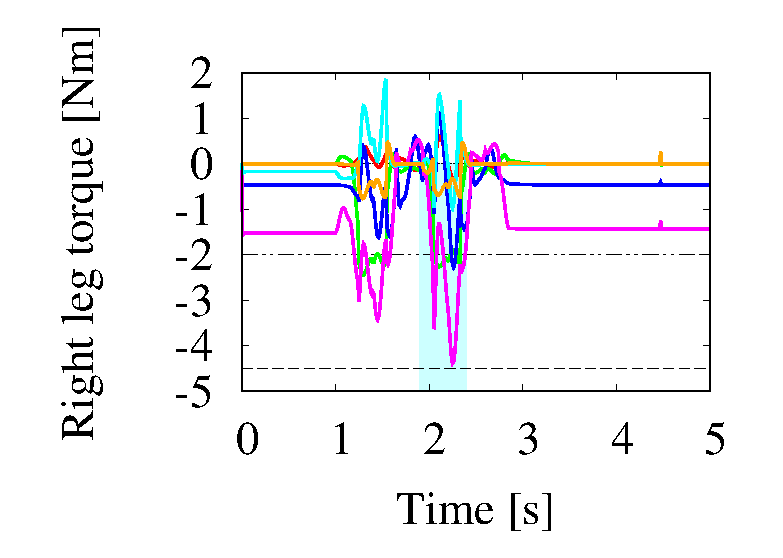
\includegraphics[width=1.0\linewidth]{./fig/original.eps}
%     \footnotesize{\hspace{30pt}(a)}
%   \end{minipage}
%   \begin{minipage}{0.5\linewidth}
%     \centering
%     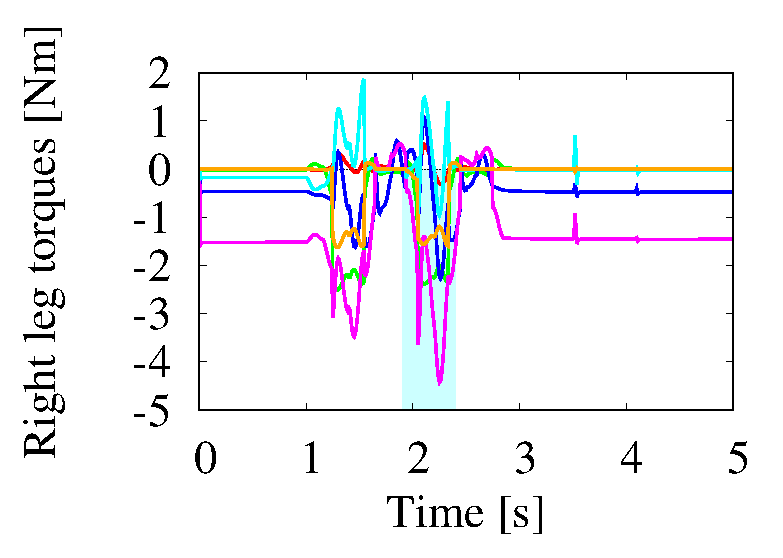
\includegraphics[width=1.0\linewidth]{./fig/0511.eps}
%     \footnotesize{\hspace{30pt}(b)}
%   \end{minipage}
%   \caption{Simuration result of torque.}
%   \label{fig:CHT7}
% \end{figure}

%#############################################################################
% ############################################################################
% \begin{figure}[h]
%   \begin{minipage}{0.5\linewidth}
%     \centering
%     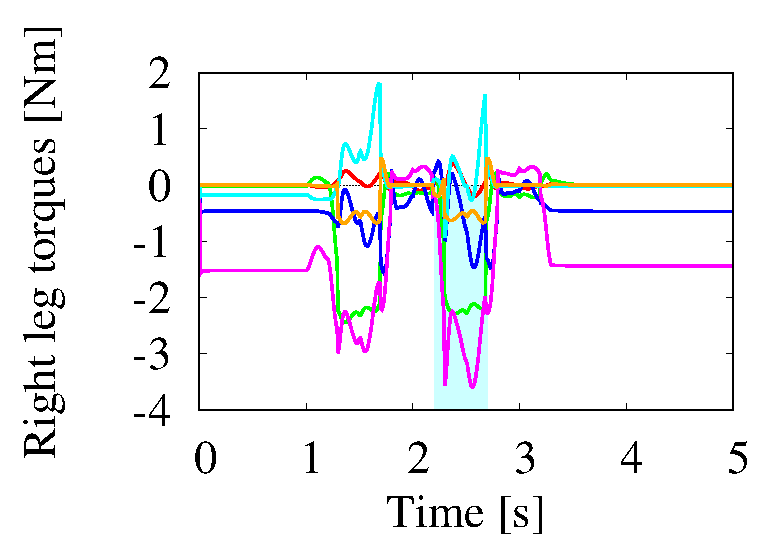
\includegraphics[width=1.0\linewidth]{./fig/0503.eps}
%     \footnotesize{\hspace{30pt}(a)}
%   \end{minipage}
%   \begin{minipage}{0.5\linewidth}
%     \centering
%     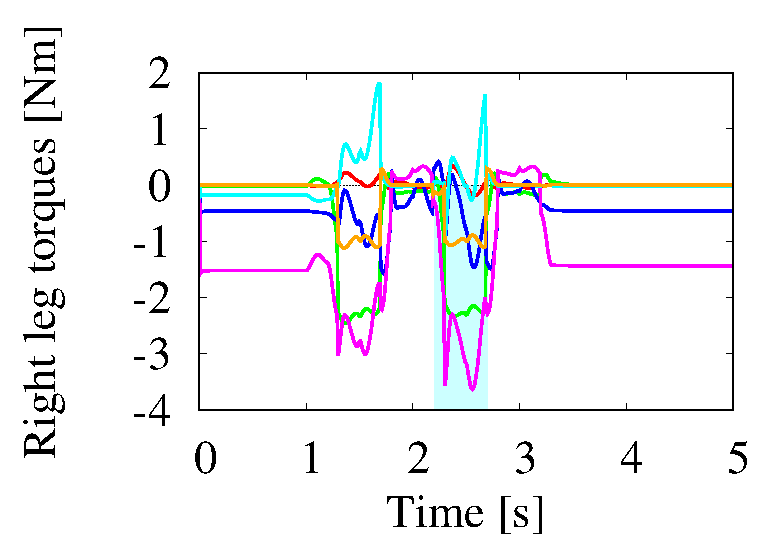
\includegraphics[width=1.0\linewidth]{./fig/0513.eps}
%     \footnotesize{\hspace{30pt}(b)}
%   \end{minipage}
%   \caption{Simuration result of torque.}
%   \label{fig:CHT8}
% \end{figure}
   %    #############################################################################
\subsection{動歩行}
Fig.~\ref{fig:CHT9}より片脚支持期間の際にCoPがBoSの外にあることがわかる.$T_{step}$を0.5 sおよび0.7 sの際にVRP offset 0.02,0.024とし動歩行を実現させた. 
% \begin{table}[b]
%   \centering
%   \caption{Step period and VRP offset.}
%   \vspace{-2mm}
%   \begin{tabular}[t]{|c||c|c|}
%     \hline
%     $T_{step}$ [s]& 0.5 & 0.7  \\ \hline
%     $T_{DS}$ [s]& 0.1 & 0.1 \\ \hline
%     $T_{SS}$ [s]& 0.4 & 0.6  \\ \hline
%     offset [m] & 0.02 & 0.024  \\\hline
%    $\tau_{6,\rm{max}}$ [Nm] & -1.30 & -1.49\\\hline
%   \end{tabular}
%   \label{tab:table9}
% \end{table}

% \begin{figure}[b]
%   \begin{minipage}{0.18\hsize}
%         \hspace{2mm}
%       \end{minipage}
% \begin{minipage}{0.33\linewidth}
%     \centering
%     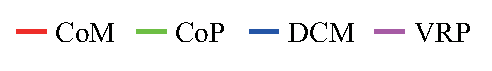
\includegraphics[width=1.0\linewidth]{./fig/key4.eps}
%   \end{minipage}
%    \begin{minipage}{0.18\hsize}
%         \hspace{2mm}
%       \end{minipage}
%   \begin{minipage}{0.48\linewidth}
%     \centering
%     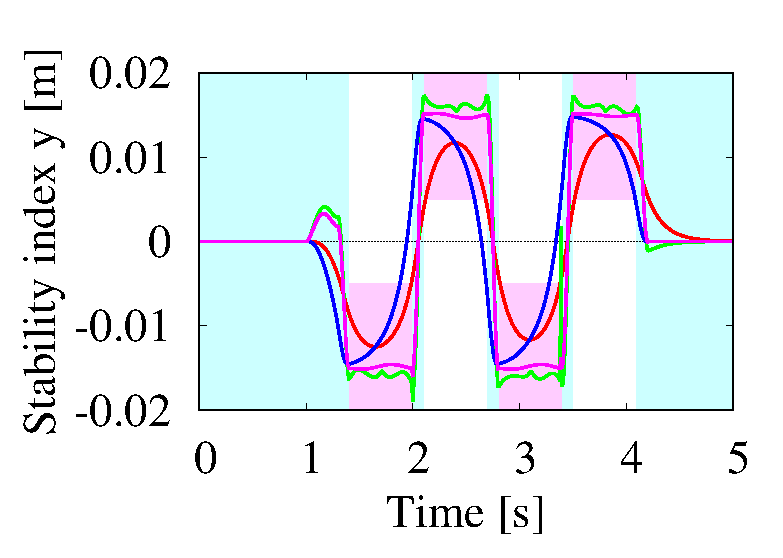
\includegraphics[width=1.0\linewidth]{./fig/No1.eps}
%     \footnotesize{\hspace{30pt}(a)}
%   \end{minipage}
%   \begin{minipage}{0.48\linewidth}
%     \centering
%     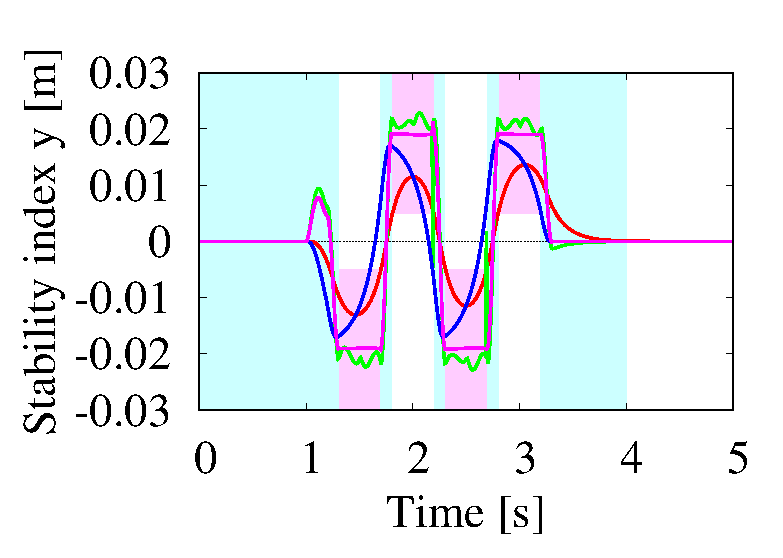
\includegraphics[width=1.0\linewidth]{./fig/No2.eps}
%     \footnotesize{\hspace{30pt}(b)}
%   \end{minipage}
%   \caption{Simuration result of torque.}
%   \label{fig:CHT9}
% \end{figure}
\subsection{まとめ}
歩幅を小さくすることでトルクを抑さえることが可能であるが,ステップ周期を変えた際との変化量を比較すると,周期を変化させた際のトルクの減少量よりも小さい値である.よって,以降ステップ周期によりトルクを抑えることを目指す.また,$T_{SS}$を長くすることで最もトルクを抑えることができる.
重心高さを高くし,トルクを抑えるさえること試みた.しかし現在の重心高さは0.24 mであり,重心高さをさらに上げると関節が特異点に入ってしまうことがわかった.%よって,現状の重心高さが適していると考えられる.
% \section{結言}
% 現状として,トルクを抑えることができたが,各関節の干渉有無の確認ができていない.そこで,実機モデルを用いた各関節の干渉確認を行い,実機実験による静歩行の実現を目指す.
% #############################################################################
% \section{今後の研究}
% 現状として,トルクを抑えることができた.しかし,各関節の干渉有無の確認ができていない.そこで,実機モデルを用いて,各関節の干渉確認を行う.また,実機実験による静歩行の実現を目指す.
   %    今まで使われていたHOAP--2の制御図をFig.~\ref{fig:block1},今後用いる制御図をFig.~\ref{fig:block}に示した.
%################################################################
% \begin{table}[h]
%   \centering
%   \caption{Joint allowable torques.}
%   \vspace{-2mm}
%   \begin{tabular}[t]{|c||c|c|c|c|c|c|}
%     \hline
%     Joint number & 1 & 2 & 3 & 4 & 5 & 6\\ \hline\hline
%     Regular use [Nm]& 1.5 & 2.0 & 1.5 & 2.0 & 1.5 & 1.5\\ \hline
%     Instantaneous [Nm]& 3.0& 4.5 & 3.0 & 4.5 & 3.0 & 3.0\\ \hline
%   \end{tabular}
%   \label{tab:table1}
% \end{table}
   %    ##################################################################
\begin{table}[h]
  \centering
  \caption{Step periods for comparison of $T_{step}$ .}
  \vspace{-2mm}
  \begin{tabular}[t]{|c||c|c|}
    \hline
    $Tstep$ [s]& 0.6 & 0.8 \\ \hline
    $T_{DS}$ [s]& 0.3 & 0.4 \\ \hline
    $T_{SS}$ [s]& 0.3 & 0.4 \\ \hline
    % $\tau_{4,\rm{max}}$ [Nm] & -4.50 & -3.72 \\\hline
  \end{tabular}
  \label{tab:table2}
\end{table}
   %    ###################################################################
\begin{table}[h]
  \centering
  \caption{Step periods for comparison of $T_{SS}$ .}
  \vspace{-2mm}
  \begin{tabular}[t]{|c||c|c|}
    \hline
    $Tstep$ [s]& 0.5 & 0.7 \\ \hline
    $T_{DS}$ [s]& 0.2 & 0.2 \\ \hline
   $T_{SS}$ [s]& 0.3 & 0.5 \\ \hline
    % $\tau_{4,\rm{max}}$ [Nm] & -4.49 & -3.55 \\\hline
  \end{tabular}
  \label{tab:table4}
\end{table}
   %    #############################################################
\begin{table}[h]
  \centering
  \caption{Strides for comparison of strides .}
  \vspace{-2mm}
  \begin{tabular}[t]{|c||c|c|}
    \hline
  stride [m]& 0.08 & 0.06 \\\hline 
   % $\tau_{4,\rm{max}}$ [Nm] & -4.50 & -4.04 \\\hline
  \end{tabular}
  \label{tab:table5}
\end{table}
% ####################################################################
\begin{figure}[h]
  \begin{minipage}{0.5\linewidth}
    \centering
    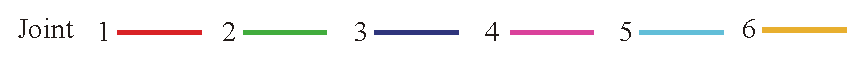
\includegraphics[width=1.0\linewidth]{./fig/key6leg.eps}
  \end{minipage}
   \begin{minipage}{0.001\hsize}
        \hspace{0.02mm}
      \end{minipage}
  \begin{minipage}{0.28\linewidth}
    \centering
    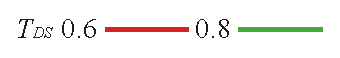
\includegraphics[width=1.0\linewidth]{./fig/keyV2.eps}
 \end{minipage}
    \begin{minipage}{0.001\hsize}
        \hspace{0.02mm}
      \end{minipage}
  \begin{minipage}{0.48\linewidth}
    \centering
    \includegraphics[width=1.0\linewidth]{./fig/original.eps}
     \footnotesize{\hspace{30pt}(a)}
  \end{minipage}
    \begin{minipage}{0.49\linewidth}
    \centering
    \includegraphics[width=1.0\linewidth]{./fig/TDS.eps}
     \footnotesize{\hspace{30pt}(b)}
  \end{minipage}
   \begin{minipage}{0.1\hsize}
        \hspace{0.02mm}
      \end{minipage}
   \begin{minipage}{0.28\linewidth}
     \centering
    \includegraphics[width=1.0\linewidth]{./fig/keyV1.eps}
  \end{minipage}
   \begin{minipage}{0.1\hsize}
        \hspace{0.02mm}
      \end{minipage}
  \begin{minipage}{0.33\linewidth}
    \centering
    \includegraphics[width=1.0\linewidth]{./fig/keyV3.eps}
  \end{minipage}
   \begin{minipage}{0.001\hsize}
        \hspace{0.02mm}
      \end{minipage}
   \begin{minipage}{0.49\linewidth}
    \centering
    \includegraphics[width=1.0\linewidth]{./fig/TSS.eps}
     \footnotesize{\hspace{30pt}(c)}
  \end{minipage}
   \begin{minipage}{0.49\linewidth}
    \centering
    \includegraphics[width=1.0\linewidth]{./fig/hohaba.eps}
     \footnotesize{\hspace{30pt}(d)}
  \end{minipage}
  \caption{Simulation results of torques:(a)right leg joints, (b) $T_{step}$ are 0.6 s and 0.8 s, (c) $T_{SS}$ are 0.3 s and 0.5 s and (d) strides are 0.08 m and 0.06 m .}
  \label{fig:CHT1}
\end{figure}
% ##################################################
\begin{figure}[h]
  \begin{minipage}{0.18\hsize}
        \hspace{0.2mm}
      \end{minipage}
\begin{minipage}{0.33\linewidth}
    \centering
    \includegraphics[width=1.0\linewidth]{./fig/key4.eps}
  \end{minipage}
   \begin{minipage}{0.18\hsize}
        \hspace{0.2mm}
      \end{minipage}
  \begin{minipage}{0.48\linewidth}
    \centering
    \includegraphics[width=1.0\linewidth]{./fig/No1.eps}
    \footnotesize{\hspace{30pt}(a)}
  \end{minipage}
  \begin{minipage}{0.48\linewidth}
    \centering
    \includegraphics[width=1.0\linewidth]{./fig/No2.eps}
    \footnotesize{\hspace{30pt}(b)}
  \end{minipage}
  \caption{Choreonoid simulation of dynamic straight walking on a flat floor. The
blue/pink areas signify the double support and single support respectively .}
  \label{fig:CHT9}
\end{figure}
\section{結言}
CHTによる軌道生成を行うと共に,$T_{step}$,$T_{SS}$および歩幅を変えることでトルクの検証を行った.結果として,片脚支持期間において最もトルクが大きくなっていることから,$T_{SS}$を長くすることで脚部のトルクを抑えることが可能であることがわかった.また,現状としてトルクを抑えることができたが,各関節の干渉有無の確認ができていない.そこで,実機モデルを用いた各関節の干渉確認を行う.その後,実機実験による静歩行および動歩行を目指す.
% \begin{table}[b]
%   \centering
%   \caption{Step period and VRP offset.}
%   \vspace{-2mm}
%   \begin{tabular}[t]{|c||c|c|}
%     \hline
%     $T_{step}$ [s]& 0.5 & 0.7  \\ \hline
%     $T_{DS}$ [s]& 0.1 & 0.1 \\ \hline
%     $T_{SS}$ [s]& 0.4 & 0.6  \\ \hline
%     offset [m] & 0.02 & 0.024  \\\hline
%    $\tau_{6,\rm{max}}$ [Nm] & -1.30 & -1.49\\\hline
%   \end{tabular}
%   \label{tab:table9}
% \end{table}


   %    \section{緒言}
% \label{sec:intro}
% % ##############################################
% 本稿では,\TeX~講習会を行うにあたり最低限必要な項目について説明を行う.
% 発表資料作成方法についてはRLS-Wikiを参考にされたい.


% % ##############################################
% \section{箇条書き}
% \label{sec:itemizeFormat}
% % ##############################################
% \subsection{itemizeの書式}
% \label{subsec:itemize}
% % ##############################################
% \begin{itemize}
% \item 箇条書き1
% \item 箇条書き2
% \item 箇条書き3
% \end{itemize}


% % ##############################################
% \subsection{enumerateの書式}
% \label{subsec:enumerate}
% % ##############################################
% \begin{enumerate}
% \item 数値付き箇条書き1
% \item 数値付き箇条書き2
% \item 数値付き箇条書き3
% \end{enumerate}


% % ##############################################
% \subsection{descriptionの書式}
% \begin{description}
%   % ##############################################
% \item[Phase I]
% \item[Phase II]
% \item[Phase III]
% \end{description}


% % ##############################################
% \section{画像の挿入}
% \label{sec:image}
% % ##############################################
% 本章では,画像の挿入方法について説明を行う.
% 画像ファイルは基本的にepsファイルを用いるが,
% 写真を挿入する場合はjpgファイルを用いる.


% % ##############################################
% \subsection{図の挿入}
% \label{subsec:figure}
% % ##############################################
% 図を単体で挿入する場合,
% 複数の図を一つのFigとして示す場合,
% ファイルの枠組みを無視して図を挿入する場合をそれぞれ
% Fig.~\ref{fig:model},
% Fig.~\ref{fig:minipage},
% Fig.~\ref{fig:forcedInsert}に示す.
% % \fig{model}
% % \fig{minipage}
% % \fig{forcedInsert}
% % ==============================================
% \begin{figure}[t]
%   % 図を挿入場所は b:bottom, h:hear, t:top, p:pageを用いて調整
%   \centering
%   \includegraphics[width=0.8\linewidth]{./fig/hoap2model.eps}
%   % 画像ファイルの相対パス
%   \caption{Sample figure.}
%   % 画像のキャプション
%   \label{fig:model}
%   % 文中で参照する場合に用いる
% \end{figure}
% % ..............................................
% % ==============================================
% \begin{figure}[t]
%   \begin{minipage}{0.45\linewidth}
%     \centering
%     \includegraphics[width=0.95\linewidth]{./fig/result1.eps}
%     \footnotesize{\hspace{30pt}(a)}
%   \end{minipage}
%   \begin{minipage}{0.45\linewidth}
%     \centering
%     \includegraphics[width=0.95\linewidth]{./fig/result2.eps}
%     \footnotesize{\hspace{30pt}(b)}
%   \end{minipage}
%   \caption{Simulation results: (a) joint torque and (b) angular momentum.}
%   \label{fig:minipage}
% \end{figure}
% % ..............................................
% % ==============================================
% \begin{figure*}[t]
%   \begin{minipage}{0.333\linewidth}
%     \centering
%     \includegraphics[width=1.0\linewidth]{./fig/hoap2model.eps}
%     \footnotesize{(a)}
%   \end{minipage}
%   \begin{minipage}{0.333\linewidth}
%     \centering
%     \includegraphics[width=1.0\linewidth]{./fig/hoap2model.eps}
%     \footnotesize{(b)}
%   \end{minipage}
%   \begin{minipage}{0.333\linewidth}
%     \centering
%     \includegraphics[width=1.0\linewidth]{./fig/hoap2model.eps}
%     \footnotesize{(c)}
%   \end{minipage}
%   \caption{Sample figure 3: (a) HOAP-2 1, (b) HOAP-2 2 and (c) HOAP-2 3.}
%   \label{fig:forcedInsert}
% \end{figure*}
% % ..............................................


% % ##############################################
% \subsection{写真の挿入}
% \label{sec:photos}
% % ##############################################
% 写真を挿入する方法をFig.~\ref{fig:photoData}に示す.
% ただし,事前に写真データに対してextractbbコマンドを実行し,
% バウンディングを作成しておく必要がある.
% また,dviファイルに写真は表示されないことに注意されたい.
% % ==============================================
% \begin{figure}[t]
%   \centering
%   \includegraphics[width=0.8\linewidth]{./photos/homeRobot.jpg}
%   \caption{Robot photo.}
%   \label{fig:photoData}
% \end{figure}
% % ..............................................


% % ##############################################
% \section{表の挿入}
% \label{sec:table}
% % ##############################################
% 表のサンプルをTable~\ref{tab:sample}に示す.
% % ==============================================
% \begin{table}[b]
%   \centering
%   \caption{Format sample.}
%   \vspace{-3mm}
%   \begin{tabular}[t]{|c|c|}
%     \hline
%     Item~[unit] & Value \\ \hline \hline
%     item1 & value1 \\ \hline
%     item2 & value2 \\ \hline
%   \end{tabular}
%   \label{tab:sample}
% \end{table}
% % ..............................................


% % ##############################################
% \section{式の挿入}
% \label{sec:formula}
% % ##############################################
% 本章では,数式を記述する際に必要となる最低限の内容を説明する.


% % ##############################################
% \subsection{太文字・イタリック文字}
% \label{subsec:boldAndItalic}
% % ##############################################
% 変数がベクトルや行列等多次元の量を表す場合においては太文字を用いる.以下に一例を示す.
% \begin{itemize}
% \item スカラー\\
%   $a$
% \item ベクトル\\
%   $\bm{x}$
% \item 行列\\
%   $\bm{A}$
% \end{itemize}


% % ##############################################
% \subsection{文中における式の表記}
% \label{subsec:inDoc}
% % ##############################################
% 文中で数式を記述する場合は,$f = ma$とする.
% % $$内に囲まれた文字が数式として処理される.


% % ##############################################
% \subsection{別行立ての数式}
% \label{subsec:anothorLine}
% % ##############################################
% 独立の行に数式を記述する場合は以下の方法を用いる.
% % align以外に同等の処理行う命令が存在するが,基本的にはalignを使うことで問題はない.
% % 他の命令(equation, gather等)については各自参照されたい.
% \begin{align}
%   f &= ma \label{eq:newton}\\
%   E &= mc^{2} \label{eq:einstein}
% \end{align}


% % ##############################################
% \subsection{行列およびベクトル}
% \label{subsec:matrixAndVector}
% % ##############################################
% 行列を記述する場合は,太文字かつ大文字として変数を表現する.
% 一例として回転変換行列を以下に示す.
% \begin{align}\label{eq:matrix}
%   ^{0}_{1}\bm{R} = \bm{R}_{z,\theta} =
%   \begin{bmatrix}
%     \cos{\theta} & -\sin{\theta} & 0 \\
%     \sin{\theta} & \cos{\theta} & 0 \\
%     0 & 0 & 1
%   \end{bmatrix}
% \end{align}
% 上付き文字および下付き文字に関しては,(\ref{eq:matrix})に示す方法で表記する.
% また,$cos$は,$\cos$として表記する.
% \par
% 文中においてベクトルの成分表記を行う場合は$\bm{r} = [x~y~z]^{T}$とする.


% % ##############################################
% \subsection{分数}
% \label{subsec:fraction}
% % ##############################################
% 別行立ての数式における分数の書き方を以下に示す.
% \begin{align}
%   \frac{a}{b}
% \end{align}
% また,文中での表記は,$a/b$とする.


% % ##############################################
% \subsection{応用例}
% \label{subsec:equation}
% % ##############################################
% 以上の数式の書き方を基に,以下に運動方程式を示す.
% % ==============================================
% \begin{align}
%   \begin{bmatrix}
%     {\bm {M}}_{A} & {\bm {M}}_{Al} \\
%     {\bm {M}}_{Al}^{T} & {\bm {M}}_{l}
%   \end{bmatrix}
%   \begin{bmatrix}
%     {\dot {\cal {V}}}_{A} \\
%     {\ddot {\bm {\theta}}}
%   \end{bmatrix}
%   &+
%   \begin{bmatrix}
%     {\cal {C}}_{A} \\
%     {\bm {c}}_{l}
%   \end{bmatrix}
%   +
%   \begin{bmatrix}
%     {\cal {G}}_{A} \\
%     {\bm {g}}_{l}
%   \end{bmatrix} \notag \\
%   &=
%   \begin{bmatrix}
%     {\cal {F}}_{A} \\
%     {\bm {\tau}}
%   \end{bmatrix}
%   +
%   \begin{bmatrix}
%     {\bm {P}}_{B} \\
%     {\bm {J}}_{B}^{T}
%   \end{bmatrix}
%   {\cal {F}}_{B}
%   \label{eq:ABundou}
% \end{align}
% % ..............................................

% ${\bm {M}}_{A} \in {\Re}^{m \times m}$はA部周りにおけるシステム全体の慣性行列を示す.

% % % ##############################################
% % \section{アルゴリズム}
% % \label{sec:algorithm}
% % % ##############################################

% % ##############################################
% \section{文献の参照}
% \label{sec:reference}
% % ##############################################
% \footnotesize
% \begin{thebibliography}{10}
%   \vspace{1truemm}
% \bibitem{armMotion} {
%     S.~Kuindersma,~R.~Grupen,~A.~Barto, 
%     ``Learning Dynamic Arm Motions for Postural Recovery,'' 
%     {\it IEEE Int. Conf. on Humanoids}, 
%     pp.~7-12,~2011.
%   }
% \bibitem{test}{
%     三枝桂祐,
%     “ダイレクトドライブモータを用いた動作解析環境の構築と
%     突発的な外力に対する人間の姿勢運動戦略の解析”,
%     東京都市大学~ロボティックライフサポート研究室,
%     pp.~65-85,~2013.
%   }
% \end{thebibliography}
%%%%%%%%%%%%%%%%%%%%%%%%%%%%%%%%%%%%%%%%%%%%%%%%%%%%%%%%%%%%%%%%%%%%%%%% 
% 
%% checklist
\newpage
% *******************************************************************************
% The command of check list
% Arguments are 0, 1 and 2.
% 0 is a blank. 1 is a check mark. 2 is a hyphen.
% *******************************************************************************
\newcommand{\listcheck}[4]{
  \ifcase #1 &\or
  $\surd$& \or --&\fi
  \ifcase #2 &\or
  $\surd$& \or --&\fi
  \ifcase #3 &\or
  $\surd$& \or --&\fi
  \ifcase #4 \or
  $\surd$ \or --\fi
}
% *******************************************************************************
\begin{table*}[htbp]
  \centering
  \caption{The referee of seminar document and power point.}\label{tab.check}
  \begin{tabular}{|c|c|c||c|c|c|}\hline
    \makebox[30pt][c]{Number}&\makebox[25pt][c]{Grade}&\makebox[155pt][c]{Name}&
    \makebox[30pt][c]{Number}&\makebox[25pt][c]{Grade}&\makebox[155pt][c]{Name}\\\hline

    % number&grade&name&&
    % number&grade&name\\\hline
    1 & & & 4 &  & \\\hline
    2 & & & 5 &  & \\\hline
    3 & & &6 &  & \\\hline
  \end{tabular}
\end{table*}
\begin{table*}[htbp]
  \centering
  \caption{The check points of tex.}\label{tab.list}
  \begin{tabular}{|c|c|c|c|c|}\hline
    \makebox[335pt][c]{Check Points}&\makebox[25pt][c]{Myself}&\makebox[25pt][c]{1}
    &\makebox[25pt][c]{2}&\makebox[25pt][c]{3}\\\hline
    % Check Points&myself&1&2&3\\\hline
    % *******************************************************************************
    % tex
    % *******************************************************************************
    題目の単語の頭文字は大文字(4文字未満の前置詞,冠詞は小文字)
    &\listcheck{1}{1}{0}{0}\\\hline
    苗字と名前の間は半角スペース
    &\listcheck{1}{1}{0}{0}\\\hline
    英語のフォントは Times New Roman
    &\listcheck{1}{1}{0}{0}\\\hline
    図やグラフを並べた際に図の大きさがそろっている
    &\listcheck{1}{1}{0}{0}\\\hline
    単位と数字の間にスペース 例:$\bigcirc$~10~mm,$\times$~10mm
    &\listcheck{2}{2}{0}{0}\\\hline
    単位は斜体にしない 例:$\bigcirc$~10~mm,$\times$~10~$mm$
    &\listcheck{1}{1}{0}{0}\\\hline
    変数に対する単位には[~]を付ける 例:$b$~[m], 5 m
    &\listcheck{1}{1}{0}{0}\\\hline
    文中や式中の変数の書体はイタリック,定数の書体はブロック
    &\listcheck{1}{1}{0}{0}\\\hline
    日本語文中の「(」,「)」,「,」,「.」は全角
    &\listcheck{1}{1}{0}{0}\\\hline
    % 一つ,二つ,三次元などは漢数字
    % &\listcheck{0}{0}{0}{0}\\\hline
    グラフ,文中の (a) などの括弧は半角
    &\listcheck{1}{1}{0}{0}\\\hline
    文中の数式関係の括弧は半角
    &\listcheck{1}{1}{0}{0}\\\hline
    比較検証の場合,同じ条件下での結果である
    &\listcheck{1}{1}{0}{0}\\\hline
    背景と目的がつながっている
    &\listcheck{1}{1}{0}{0}\\\hline
    省略されている単語の前に省略前の単語がある 例:Center of Mass(CoM)
    &\listcheck{1}{1}{0}{0}\\\hline
    参考文献の書き方が正しい
    &\listcheck{2}{2}{0}{0}\\\hline
    セミナー3日前に第一版のチェックを受けた
    &\listcheck{2}{2}{0}{0}\\\hline
    セミナー当日正午までに最終版のチェックを受けた
    &\listcheck{1}{1}{0}{0}\\\hline
    % *******************************************************************************
    % 参考文献
    % *******************************************************************************
    % 学会誌(注意:題名と学会誌名の後の「,」は全角)&&&&\\
    % 人名,``題名'',学会誌名,\verb*|vol. 2,no. 1,pp. 12--18, 2008.|
    % &-&&&\\\hline
    % 公演論文(日本の場合発表番号と年の間の「,」と文末の「.」だけ半角)&&&&\\
    % 人名,人名,``題名'',公演論文集名,発表番号\verb*|, 2009.|
    % &-&&&\\\hline
    % 卒論・修論(文末の「.」だけ半角)&&&&\\
    % 執筆者(記者名 \verb*|\ | 訳),``題目'',修士論文,&&&&\\
    % 東京都市大学工学部機械システム工学科,2009.
    % &-&&&\\\hline
    % 本(注意:「``」,「''」と文末の「.」以外は全角)&&&&\\
    % 著者名,``本の題名'',出版社,出版年,pp200--205.&&&&\\
    % (引用ページがない場合は「出版年.」)
    % &-&&&\\\hline
    % ホームページ(() 内は最後にそのページを見た日)&&&&\\
    % 作者名(わかる場合のみ).(\verb*|2010,\ Dec.\ 12|)ホームページ名&&&&\\
    % \verb*|\ [Online].\ Available:\url{|ホームページの URL\verb*|}|
    % &-&&&\\\hline
    % IEEEに基づく書き方例(題名,を「``」,「''」でくくる)&&&&\\
    % J. K. Author, ``Title of chapter in the book,''&&&&\\
    % in Title of His Published Book, xth ed. City of Publisher,&&&&\\
    % Country if not USA: Abbrev. of Publisher, year, ch. x,&&&&\\
    % sec. x, pp. xxx-xxx.&&&&\\
    % &-&&&\\\hline
  \end{tabular}
\end{table*}

\begin{table*}
  \centering
  \caption{The check points of ppt.}\label{tab.ppt}
  \begin{tabular}{|c|c|c|c|c|}\hline
    % *******************************************************************************
    % ppt
    % *******************************************************************************
    Check Points&\makebox[25pt][c]{Myself}&\makebox[25pt][c]{4}
    &\makebox[25pt][c]{5}&\makebox[25pt][c]{6}\\\hline

    日本語のフォントは MS~Pゴシック,英語は Times New Roman
    &\listcheck{0}{0}{0}{0}\\\hline
    真っ白なスライドデザインは使用しない
    &\listcheck{0}{0}{0}{0}\\\hline
    左右の余白が最低グリッド1マス分空いている
    &\listcheck{0}{0}{0}{0}\\\hline
    文字は単文にし,「.」は使用していない
    &\listcheck{0}{0}{0}{0}\\\hline
    文章の書き出しや,図表はページの中でそろえて配置
    &\listcheck{0}{0}{0}{0}\\\hline
    文字のサイズは四種類まで(大題,小題,本文,図のキャプション)
    &\listcheck{0}{0}{0}{0}\\\hline
    文字を見やすくするため,フォントサイズは 20 point 以上
    &\listcheck{0}{0}{0}{0}\\\hline
    % 強調のために赤と青の色を用いている (赤は瞬間的に,青は持続的に記憶される)
    % &\listcheck{0}{0}{0}{0}\\\hline
    矢印の色と位置がそろってる(色は単色とし,全てのスライドで同じ色を用いる)
    &\listcheck{0}{0}{0}{0}\\\hline
    写真,グラフ,表,動画を用いて見やすいスライドになっている
    &\listcheck{0}{0}{0}{0}\\\hline
    各スライドの発表時間が約30$\sim$60~秒になるような構成
    &\listcheck{0}{0}{0}{0}\\\hline
    「ご清聴ありがとうございました」を使っている(ご静聴ではない)
    &\listcheck{0}{0}{0}{0}\\\hline
    セミナー前にチェックを受けた
    &\listcheck{0}{0}{0}{0}\\\hline
  \end{tabular}
\end{table*}

%% Local Variables:
%% mode: japanese-latex
%% TeX-master: t
%% End:

%%%%%%%%%%%%%%%%%%%%%%%%%%%%%%%%%%%%%%%%%%%%%%%%%%%%%%%%%%%%%%%%%%%%%%%% 
% % 
% \clearpage
% \section{rlsTex内に定義されたマクロの使用例}
% texs直下にあるrlsTex/mydef内で定義されているマクロの使用例です.
% texの使い方に慣れてきたらマクロを自分で設定して使ってみてください.
% \subsection{浮遊ベースロボットの運動方程式}
% \bal[eom]{
%   \bmMM[exp2]\ddbmqM[exp2] + \bmcM[exp2] + \bmgC[exp2] = \bmQ[exp2] + \bmJcM[exp2][T]\obmcalFc
% }
% \cite{kajita2003}

% \subsection{図}
% \bfig{h}[result]{
%   \bmpnsc{t}{1.}{
%     \ig{.3}{key/workKey.eps}
%   }
%   \bmpsc{h}{1.}{
%     \ig{.7}{model/skeletonA7.eps}
%   }
% }{
%   Caption
% }

% \subsection{bibTex}

%% reference
\bibliographystyle{junsrt}
%\input{\rlsbib/wrapper/humanoid}

\end{document}

Local Variables:
mode: japanese-latex
TeX-master: t
End:
